% --- Progetto Basi di Dati ---
\documentclass[a4paper, 12pt]{article} % Qui era 12pt

% --- PACKAGES ---

\usepackage[italian]{babel}
\usepackage{comment}

\usepackage{microtype}
\usepackage{graphicx}
\usepackage{wrapfig}
\usepackage{enumitem}
\usepackage{fancyhdr}

\usepackage{amsmath}

%\usepackage{paralist} % SE ATTIVO PARALIST, ITEMIZE ED ENUMERATE NON FUNZIONANO!!!

\usepackage{amsthm}
% it introduces the \newtheorem command
\usepackage{amssymb}
% new mathematical symbols
\usepackage{eucal}
% other mathematical symbols
\usepackage{gensymb}
% \degree \celsius \micro \ohm \perthousand
\usepackage{mathptmx}
% other mathematical symbols
\usepackage{latexsym}
% other mathematical symbols
\usepackage{mathtools}
% supplements amsmath
\usepackage{textcomp}
% extra symbols arrows like \textrightarrow, \texteuro, \textcelsius

\usepackage[utf8]{inputenc}
%\usepackage[utf8x]{inputenc}
%\usepackage[latin1]{inputenc}
\usepackage{listingsutf8}
%\usepackage[overload]{textcase}

\usepackage{multicol}
% Per le colonne

%\usepackage{xcolor}
% Per colorare il testo

\usepackage[table, dvipsnames]{xcolor}
% Per ulteriori colori
% Quel table serve invece per colorare le righe in tabular

\usepackage[document]{ragged2e}

\usepackage{blindtext}

\usepackage[scaled=.92]{helvet}

\usepackage{tikz}

%\usepackage{floatrow}

%\usepackage{makecell}

\usepackage[T1]{fontenc}
%\usepackage{fourier, erewhon}
\usepackage{geometry}
%\usepackage[landscape]{geometry}
\usepackage{array, caption, floatrow, tabularx, makecell, booktabs}%

\usepackage{amsfonts}

%\graphicspath{ {./images/} }
% graphicspath dice a LaTex la path della cartella dove si trovano le immagini.

\usepackage{float}

\usepackage{etoc}

\usepackage{titlesec}
%\titleformat{\section}{\normalfont\Large\bfseries\center}{}{0pt}{} % Questo serve per togliere il numero dalla section ; Qui ho aggiunto \center e ora sono centrati

%\usetikzlibrary{snakes}

\usepackage[most]{tcolorbox}

\usepackage{wasysym} % per il Checkmark boxed

\usepackage{hyperref} % per i link e i checkbox

%\usepackage{pict2e}

\usepackage{subcaption} % per subfigure


%\begin{comment}

\titleformat
{\section} % command
[display] % shape
{\normalfont\Large\bfseries\center} % format
{} % label
{-2ex} % sep %0.5ex
{
	\rule{\textwidth}{1pt} % 1 pt
	\vspace{-2pt} % 1ex
	\centering
} % before-code
[
\vspace{-2ex}% -0.5ex valori originari
\rule{\textwidth}{0.3pt} % 0.3pt
] % after-code

%\end{comment}

\begin{comment}
\titleformat{\section}[block]
{\titlerule\addvspace{4pt}\normalfont\Large\bfseries\center}
{\thesection\enspace}{0pt}{}[\vspace{2pt}\titlerule]
\end{comment}

\titleformat{\subsection}{\normalfont\large\bfseries\center}{}{0pt}{} % Questo l'ho copiato da sopra ed ho aggiunto center e ora sono centrati
\titleformat{\subsubsection}{\normalfont\large\bfseries\center\color{red}}{}{0pt}{} % Questo l'ho copiato da sopra ed ho aggiunto center e ora sono centrati
\setcounter{secnumdepth}{2} % levels under \subsection are not numbered
% secnumdepth 1 è \section 2 è \subsection
\setcounter{tocdepth}{3}    % levels under \subsubsection are not listed in the TOC
% tocdepth 1 è section 2 è subsection e 3 è subsubsection

%\usepackage{sectsty} % Se lo attivo mi metti i numerini nella section
%\sectionfont{\centering}
%\allsectionsfont{\centering}

\usepackage{diffcoeff} % per le derivate

\usepackage{pagecolor,lipsum} %pagecolor per colorare la pagina (il background)
% lo sfondo in italiano
\usepackage{ltablex}

\usepackage{multirow}

%\usepackage{systeme}

\usetikzlibrary{arrows.meta, angles}

\usetikzlibrary{chains,decorations.pathreplacing}

\usepackage[normalem]{ulem} % serve per sbarrare il testo (strikethrough), usare \sout

\usetikzlibrary{tikzmark} % per circondare gli elementi di una tabella (tabular)

\usetikzlibrary{shapes}

\usetikzlibrary{arrows,shapes.gates.logic.US,shapes.gates.logic.IEC,calc}

\tikzstyle{branch}=[fill,shape=circle,minimum size=3pt,inner sep=0pt]

%\usepackage{subfig} % serve per avere immagini una accanto all'altra

\usepackage{cancel} 

\usetikzlibrary{matrix}

\usepackage{soul}

%\usepackage{emerald}% per dalla 1-4 firma (questo mi da errore, not found)

\usepackage{frcursive}% serve per la firma finale (nelle Conclusioni)

\usepackage{inslrmin}% per la 6 firma

%\theoremstyle{definition}
%\newtheorem{definition}{\textcolor{red}{\underline{Def}:}}[section]
%\newtheorem{definition}{Def}[section]

%\theoremstyle{theorem}
%\newtheorem{theorem}{$\boxed{\text{Teorema}}$}[section] 
%\newtheorem* non accetta valori opzionali, per quelli usare newtheorem senza *
% è per questo che da errore
% se si mantiene l'errore, nella prima pagina prima del titolo verrà
% mostrato [section]

%\newtheorem{theorem}{Teorema}[section]
%\newtheoremstyle{theorem}{}{}{}{}{\color{red}\bfseries}{}{ }{}

\usepackage{pict2e}
%\usepackage{titling}

\usepackage{pdflscape}

\usepackage{alltt}
\usepackage{fancyvrb}
\usepackage{url}

\usepackage{lscape}

\usepackage{rotating} % per le figure sideways

%\usepackage[formats]{listings} % serve per il codice SQL

\hypersetup{
	colorlinks=true,
	linkcolor=black, %blue
	filecolor=magenta,      
	urlcolor=cyan,
	pdftitle={Sharelatex Example},
	bookmarks=true,
	pdfpagemode=FullScreen,
}

\definecolor{codegreen}{rgb}{0,0.6,0}
\definecolor{codegray}{rgb}{0.5,0.5,0.5}
\definecolor{codepurple}{HTML}{C42043}
\definecolor{backcolour}{HTML}{F2F2F2}
\definecolor{bookColor}{cmyk}{0,0,0,0.90}

\lstdefinestyle{mystyle}{
	inputencoding = utf8,  % Input encoding
	extendedchars = true,  % Extended ASCII
	backgroundcolor=\color{backcolour},   
	commentstyle=\color{codegreen},
	keywordstyle=\color{codepurple},
	%numberstyle=\numberstyle,
	stringstyle=\color{codepurple},
	basicstyle=\footnotesize\ttfamily,
	breakatwhitespace=false,
	breaklines=true,
	captionpos=b,
	keepspaces=true,
	numbers=left,
	numbersep=10pt,
	showspaces=false,
	showstringspaces=false,
	showtabs=false,
	literate      =        % Support additional characters
	{á}{{\'a}}1  {é}{{\'e}}1  {í}{{\'i}}1 {ó}{{\'o}}1  {ú}{{\'u}}1
	{Á}{{\'A}}1  {É}{{\'E}}1  {Í}{{\'I}}1 {Ó}{{\'O}}1  {Ú}{{\'U}}1
	{à}{{\`a}}1  {è}{{\`e}}1  {ì}{{\`i}}1 {ò}{{\`o}}1  {ù}{{\`u}}1
	{À}{{\`A}}1  {È}{{\'E}}1  {Ì}{{\`I}}1 {Ò}{{\`O}}1  {Ù}{{\`U}}1
	{ä}{{\"a}}1  {ë}{{\"e}}1  {ï}{{\"i}}1 {ö}{{\"o}}1  {ü}{{\"u}}1
	{Ä}{{\"A}}1  {Ë}{{\"E}}1  {Ï}{{\"I}}1 {Ö}{{\"O}}1  {Ü}{{\"U}}1
	{â}{{\^a}}1  {ê}{{\^e}}1  {î}{{\^i}}1 {ô}{{\^o}}1  {û}{{\^u}}1
	{Â}{{\^A}}1  {Ê}{{\^E}}1  {Î}{{\^I}}1 {Ô}{{\^O}}1  {Û}{{\^U}}1
	{œ}{{\oe}}1  {Œ}{{\OE}}1  {æ}{{\ae}}1 {Æ}{{\AE}}1  {ß}{{\ss}}1
	{ç}{{\c c}}1 {Ç}{{\c C}}1 {ø}{{\o}}1  {å}{{\r a}}1 {Å}{{\r A}}1
	{ñ}{{\~n}}1  {Ñ}{{\~N}}1  {¿}{{?`}}1  {¡}{{!`}}1
	% ¿ and ¡ are not correctly displayed if inconsolata font is used
	% together with the lstlisting environment. Consider typing code in
	% external files and using \lstinputlisting to display them instead. 
}
\lstset{style=mystyle}


% --- FINE USEPACKAGES ---

% ============================ COMMANDS =========================================



% !TeX root = ../Relazione_Basi_di_Dati_main.tex

% ============= FINE CUSTOM COMMANDS ============================================

\makeindex

\begin{document}
	
	\title{Relazione per il corso di Basi di dati}
	\author{Luca Rengo}
	\date{Maggio | Giugno | Luglio | Agosto 2021}
		
	\makeatletter
	\begin{titlepage}
		\begin{center}
			
\includegraphics[width=0.7\linewidth]{img/alma_mater_studiorum_cesena_logo.png}\\[4ex]
			{\Huge  \@title }\\[1ex] 
			\textbf{\LARGE Progetto di una base di dati per la gestione di un Aeroporto}\\[2ex] 
			%\Large A.A 2019/2020 \\
			{\large  \@author}\\[2ex] 
			{\large \@date}
		\end{center}
	\end{titlepage}

	\makeatother
	\thispagestyle{empty}
	
	% INIZIO: TABLEOFCONTENTS
	
	\let\cleardoublepage\clearpage
	\tableofcontents
	\pagenumbering{arabic}
	\setcounter{page}{2}
	%\etocsettocstyle{\subsection*{This Chapter contains:}}{\noindent\rule{\linewidth}{.4pt}}
	% C'è bisogno del package etoc
	%\chapter{Extinct Species}
	%\localtableofcontents
	
	% FINE: TABLEOFCONTENTS
	
	\fancyhf{}
	\begin{comment}
	\renewcommand{\headrulewidth}{2pt}
	\renewcommand{\footrulewidth}{1pt}
	\fancyhead[LE]{\leftmark}
	\fancyhead[RO]{\nouppercase{\rightmark}}
	\fancyfoot[LE, RO]{\thepage}
	\end{comment}
	
	% ================= INTRODUZIONE ===============================================

\newpage

\section{Introduzione}

\textsf{\small L'obiettivo del progetto è la realizzazione di una base di dati che gestisca tutte le operazioni necessarie per il corretto funzionamento ed il normale svolgimento delle attività aeroportuali.}\\
\textsf{\small Pertanto essa dovrà contenere tutti gli attori (entità) principali, quali: Passeggeri, Addetti di scalo, Addetti alla sicurezza, Equipaggi degli aerei, Controllori, Tecnici della manutenzione e coordinare le loro relazioni.}\\

% ================= ANALISI DEI REQUISITI ======================================

\section{Analisi dei Requisiti}

\subsection{Intervista}

\textsf{\small Si vuole tenere traccia di tutte le \textbf{persone} che si trovano in Aeroporto sia per lavoro che per usufruire di un servizio, memorizzando i loro Codici Fiscali, Nomi, Cognomi, Età.}\break % usufruire dei servizi

\textsf{\small Degli operatori addetti alle quotidiane attività aeroportuali, ci sono gli \textbf{Addetti di scalo}, ovvero l'\textbf{Agente di Rampa}, l'\textbf{Addetto al Check-In}, l'\textbf{Addetto all'imbarco}, l'\textbf{Addetto al Lost\&Found}, l'\textbf{Addetto al Weight and Balance}.}\break

\textsf{\small I \textbf{passeggeri} sono ritenuti tali solamente quando si trovano all'interno dell'\textbf{aereo}, altrimenti vengono considerati semplicemente \textbf{persone}.}\\
\textsf{\small Questi possono visitare i \textbf{negozi}, le \textbf{lounge}, comprare biglietti per il \textbf{volo}, essere controllati dagli \textbf{addetti alla sicurezza} e recarsi al \textbf{gate} per aspettare di salire sull'\textbf{aereo}.}\break

\textsf{\small Ogni \textbf{aereo} è di proprietà di una \textbf{compagnia aerea}, ha un \textbf{equipaggio}, viene mantenuto dai \textbf{tecnici della manutenzione}; viene curato dal \textbf{Ground Support Equipment}, ovvero da tutto il personale di terra che si occupa di caricare/scaricare il \textbf{cargo}, i bagagli, di rifornire di carburante, di elettricità, di cibo e bevande, di apparecchi igienico sanitari,ecc.. }\\

\textsf{\small E' necessario tenere in considerazione tutte le componenti di un \textbf{aereo}: \textbf{fusoliera}, \textbf{motori}, \textbf{ali}, \textbf{carrello}, \textbf{flaps}, \textbf{impennaggio}, \textbf{cabina},ecc.. per assicurare la sicurezza dei \textbf{passeggeri} e si possa procedere con il decollo.}\\

\textsf{\small Inoltre è di vitale importanza per la sicurezza e il corretto svolgimento delle operazioni tenere traccia della posizione degli \textbf{Aerei}, se sono fermi, in \textbf{manutenzione}, in partenza sulla \textbf{pista}.}\break

\textsf{\small Ogni \textbf{volo} riguarda il \textbf{tragitto} dall'aeroporto di \textbf{partenza} alla \textbf{destinazione} che deve fare un determinato \textbf{aereo} in un determinato \textbf{lasso di tempo}.Questo deve essere, in ogni singolo momento, tenuto sotto stretta osservazione e controllo da parte dei \textbf{Controllori} presso la \textbf{Torre di Controllo}.}\\

\textsf{\small Questi attraverso i \textbf{Radar}, devono continuamente coordinare il corretto flusso di navigazione degli \textbf{aerei}.}\\

\newpage

\enlargethispage{1\linewidth}

\subsection{Estrazione dei concetti principali}

\subsection{\textcolor{black}{Glossario dei Termini}}

\begin{comment}
\begin{tabular}{|c|c|c|}
	\textbf{Termine} & \textbf{Breve descrizione} & \textbf{Sinonimi} \\
	%\hline
	\textsf{\small Aereoporto} & \textsf{\small  è un'infrastruttura attrezzata per il decollo e l'atterraggio di aeromobili, per il transito dei relativi passeggeri e del loro bagaglio, per il ricovero e il rifornimento dei velivoli.} & \textsf{\small Aerodromo} \\
	
	\textsf{\small Aereoplano} & \textsf{\small velivolo impiegato come mezzo di trasporto, fornito di ali, motori e strutture che gli consentono di viaggiare nell’aria e di partire e atterrare su superfici idonee} & \textsf{\small Aereomobile, Aereo} \\
	
	\textsf{\small Pilota} & \textsf{\small Persona legalmente abilitata, con regolare brevetto, a guidare un aeromobile} & \textsf{\small } \\
	
	\textsf{\small Copilota} & \textsf{\small Chi, a bordo di un velivolo, può svolgere tutte le funzioni del pilota, fuorché quelle di pilota comandante} & \textsf{\small } \\
	
	\textsf{\small Assistente di Volo} & \textsf{\small chi assiste i passeggeri sugli aerei civili} & \textsf{\small (Hostess, Steward)} \\
	
	\textsf{\small Passeggero} & \textsf{\small Chi viaggia su nave, treno, aereo o altro mezzo di trasporto: navi da carico e per passeggeri;} & \textsf{\small } \\
	
	\textsf{\small Compagnia Aerea} & \textsf{\small è un'impresa la cui attività istituzionale consiste nel trasporto di persone o di merci mediante l'utilizzo di aeromobili.} & \textsf{\small } \\
	
	\textsf{\small Torre di Controllo} & \textsf{\small  è una struttura sopraelevata usata per le operazioni di controllo del traffico di una determinata area: controlla il traffico aereo a terra e quello che sta per atterrare.} & \textsf{\small } \\
	
	\textsf{\small Controllori del traffico aereo} & \textsf{\small sono professionisti che si occupano della fornitura dei servizi del traffico aereo negli spazi aerei di tutto il mondo, con lo scopo di mantenere un sicuro spedito e ordinato flusso del traffico aereo.} & \textsf{\small } \\
	
	\textsf{\small Pista} & \textsf{\small è una striscia di superficie di un aerodromo specificatamente attrezzata e adibita al decollo e all'atterraggio di un velivolo.} & \textsf{\small } \\
	
	\textsf{\small Via di rullaggio - taxiway} & \textsf{\small è una superficie delimitata all'interno di un aeroporto che identifica il percorso che gli aeromobili debbono percorrere per spostarsi da un punto ad un altro. Una via di rullaggio collega ad esempio le piste con l'area di stazionamento, due diverse parti dell'area di parcheggio, le piazzole di sosta e altre strutture} & \textsf{\small } \\
	
	\textsf{\small Addetto di scalo} & \textsf{\small può svolgere il compito di agente di rampa, Weight and balance più comunemente chiamato centrista, addetto al Check-In, addetto all'imbarco o addetto al Lost \& Found.} & \textsf{\small } \\
	
	\textsf{\small Agente di rampa} & \textsf{\small  svolge compiti da tramite fra l'aeromobile e tutto il resto dell'organizzazione aeroportuale, coordinando e supervisionando tutte le attività al suolo. (è un addetto di scalo)} & \textsf{\small } \\
	
	\textsf{\small Weight and Balance} & \textsf{\small  anche conosciuto con il termine W/B o Centraggio, è quel dipartimento che si occupa di bilanciare un aeromobile, sia utilizzando supporti informatici, tecnicamente definiti DCS (Departure Control System), oppure, in caso di inattività di questi sistemi, operando manualmente tale bilanciamento tramite dei documenti cartacei chiamati Loadmessage e Trimsheet, che uniti tra loro creano un Loadsheet.} & \textsf{\small } \\
	
	\textsf{\small Addetto all'accettazione / Addetto al Check-in} & \textsf{\small Ha il compito di registrare i passeggeri all'accettazione, controllare la validità dei loro documenti e visti, emettere le carte di imbarco, registrare ed etichettare i bagagli da imbarcare. Inoltre si occupa anche dell'imbarco dei passeggeri all'uscita ed è dotato di uno speciale tesserino (lasciapassare) che gli consente di entrare nelle zone sterili dell'aeroporto per compiere il suo lavoro (soprattutto al gate e sul piazzale nel caso di assistenze particolari). (è un addetto di scalo che è un impiegato)} & \textsf{\small } \\
	
	\textsf{\small Flight Dispatcher - Flight Operations Officer} & \textsf{\small  è una figura professionale designata da un operatore aeronautico, impegnato nel controllo e supervisione delle operazioni di volo, con licenza oppure no, (opportunamente qualificato in accordo all'Annesso I ICAO,) che sostiene, dà istruzioni e/o assiste l'equipaggio nella condotta sicura del volo.} & \textsf{\small } \\
	
	\textsf{\small Terminal Aeroportuale} & \textsf{\small è un edificio dell'aeroporto che permette il trasferimento dei passeggeri dal sistema di trasporto terrestre a quello aeronautico e viceversa.} & \textsf{\small } \\
	
	\textsf{\small Trattore aeroportuale - trattore aragosta} & \textsf{\small è un veicolo usato negli aeroporti per la movimentazione degli aeromobili; è usato in particolare per il pushback, cioè per spingere un aereo parcheggiato con il muso rivolto verso il terminal nel piazzale, dove potrà iniziare il suo rullaggio autonomamente.} & \textsf{\small } \\
	
	\textsf{\small Uscita aeroportuale - gate} & \textsf{\small Un'uscita aeroportuale o gate (pron. /geit/, in inglese significa letteralmente "varco") indica, in un aeroporto, la porta attraverso cui passare per imbarcarsi su un aeroplano.} & \textsf{\small } \\
	
	\textsf{\small Faro Aerodromo} & \textsf{\small ] è un faro rotante posto in prossimità di un aeroporto per facilitare ai piloti in avvicinamento l'individuazione della sua posizione.} & \textsf{\small } \\
	
	\textsf{\small Manicotto d'imbarco} & \textsf{\small detto anche passerella telescopica o pontile d'imbarco (a volte chiamato col termine inglese finger, letteralmente "dito"), è un connettore mobile chiuso, che collega un gate di un terminal aeroportuale ad un aereo.} & \textsf{\small } \\
	
	\textsf{\small } & \textsf{\small } & \textsf{\small } \\
	
	\textsf{\small } & \textsf{\small } & \textsf{\small } \\
	
\end{tabular}
\end{comment}
%\newpage
\begin{comment}
\begin{tabular}{|c|c|c|}
	\textbf{Termine} & \textbf{Breve descrizione} & \textbf{Sinonimi} \\
	\textsf{\small Aereoporto} & \textsf{\small  è un'infrastruttura attrezzata per il decollo e l'atterraggio di aeromobili, per il transito dei relativi passeggeri e del loro bagaglio, per il ricovero e il rifornimento dei velivoli.} & \textsf{\small Aerodromo} \\
\end{tabular}
\end{comment}
%\newpage

\begin{comment}
\begin{table}[htp]
	\centering
	%\caption{My caption}
	%\label{my-label}
	{\small %
		\begin{tabular}{p{.18\textwidth}p{.22\textwidth}p{.2\textwidth}p{.2\textwidth}p{.2\textwidth}}
			Detection\par Methods & Supervised/\par Semi-supervised/\par Unsupervised & Technique Used & Applications & Technology \\
			Statistical & & Gaussian-based detection & Online anomaly detection & Conventional data centres \\
			Statistical & & Gaussian-based detection & General & General \\
			Statistical & & Regression\par analysis & Globally-distributed commercial applications & Distributed, Web-based, Application \&\par System metrics \\
			Statistical & & Regression\par analysis & Web applications & Enterprise web applications and conventional data centre \\
			Statistical & & Correlation & Complex\par enterprise online applications & Distributed\par System \\
			Statistical & & Correlation & Orleans system and distributed cloud computing services & Virtualized, cloud computing and distributed system (Orleans system) \\
			Statistical & & Correlation & Hadoop,\par Olio and RUBiS & Virtualized cloud computing and distributed systems. \\
			ĘMachine\par learning & Supervised & Bayesian\par classification & Online\par application & IBM system S-distributed stream\par processing\par cluster \\
			Machine\par learning & Unsupervised & Neighbour-based technique (Local Outlier Factor algorithm) & General & Cloud\par Computing\par system \\
			Machine\par learning & Semi-supervised & Principle component analysis and Semi-supervised Decision-tree\_ & Institute-wide cloud computing environment & Cloud\par Computing \\
			Statistical & & Regression curve fitting the service time-adapted cumulative distributed function & Online\par application service & Platform and configuration agnostic \\
			& & & & 
		\end{tabular}%
	}%
\end{table}
\end{comment}
%\newpage

\begin{landscape}

\begin{table}[htp]
	\centering
	%\caption{My caption}
	%\label{my-label}
	{\small %
		\begin{tabular}{p{.18\textwidth}|p{.7\textwidth}|p{.18\textwidth}}
		\rowcolor{airforceblue}
		\textbf{\color{white}Termine} & \textbf{\color{white}Breve descrizione} & \textbf{\color{white}Sinonimi} \\
		\hline
		\textsf{\small Aereoporto} & \textsf{\small  è un'infrastruttura attrezzata per il decollo e l'atterraggio di aeromobili, per il transito dei relativi passeggeri e del loro bagaglio, per il ricovero e il rifornimento dei velivoli.} & \textsf{\small Aerodromo} \\
		\hline
		\textsf{\small Aereoplano} & \textsf{\small velivolo impiegato come mezzo di trasporto, fornito di ali, motori e strutture che gli consentono di viaggiare nell’aria e di partire e atterrare su superfici idonee} & \textsf{\small Aereomobile, Aereo} \\
		\hline
		\textsf{\small Pilota} & \textsf{\small Persona legalmente abilitata, con regolare brevetto, a guidare un aeromobile} & \textsf{\small } \\
		\hline
		\textsf{\small Copilota} & \textsf{\small Chi, a bordo di un velivolo, può svolgere tutte le funzioni del pilota, fuorché quelle di pilota comandante} & \textsf{\small } \\
		\hline
		\textsf{\small Assistente di Volo} & \textsf{\small chi assiste i passeggeri sugli aerei civili} & \textsf{\small (Hostess, Steward)} \\
		\hline
		\textsf{\small Passeggero} & \textsf{\small Chi viaggia su nave, treno, aereo o altro mezzo di trasporto: navi da carico e per passeggeri;} & \textsf{\small } \\
		\hline
		\textsf{\small Compagnia Aerea} & \textsf{\small è un'impresa la cui attività istituzionale consiste nel trasporto di persone o di merci mediante l'utilizzo di aeromobili.} & \textsf{\small } \\
		\hline
		\textsf{\small Torre di Controllo} & \textsf{\small  è una struttura sopraelevata usata per le operazioni di controllo del traffico di una determinata area: controlla il traffico aereo a terra e quello che sta per atterrare.} & \textsf{\small } \\
		\hline
		\textsf{\small Controllori del traffico aereo} & \textsf{\small sono professionisti che si occupano della fornitura dei servizi del traffico aereo negli spazi aerei di tutto il mondo, con lo scopo di mantenere un sicuro spedito e ordinato flusso del traffico aereo.} & \textsf{\small } \\
		\hline
		\textsf{\small Pista} & \textsf{\small è una striscia di superficie di un aerodromo specificatamente attrezzata e adibita al decollo e all'atterraggio di un velivolo.} & \textsf{\small } \\
		\hline
		\textsf{\small Via di rullaggio - taxiway} & \textsf{\small è una superficie delimitata all'interno di un aeroporto che identifica il percorso che gli aeromobili debbono percorrere per spostarsi da un punto ad un altro. Una via di rullaggio collega ad esempio le piste con l'area di stazionamento, due diverse parti dell'area di parcheggio, le piazzole di sosta e altre strutture} & \textsf{\small } \\
		\hline
		\textsf{\small Addetto di scalo} & \textsf{\small può svolgere il compito di agente di rampa, Weight and balance più comunemente chiamato centrista, addetto al Check-In, addetto all'imbarco o addetto al Lost \& Found.} & \textsf{\small } \\
		\hline
		\textsf{\small Agente di rampa} & \textsf{\small  svolge compiti da tramite fra l'aeromobile e tutto il resto dell'organizzazione aeroportuale, coordinando e supervisionando tutte le attività al suolo. (è un addetto di scalo)} & \textsf{\small } \\
		\hline
		\textsf{\small Weight and Balance} & \textsf{\small  anche conosciuto con il termine W/B o Centraggio, è quel dipartimento che si occupa di bilanciare un aeromobile, sia utilizzando supporti informatici, tecnicamente definiti DCS (Departure Control System), oppure, in caso di inattività di questi sistemi, operando manualmente tale bilanciamento tramite dei documenti cartacei chiamati Loadmessage e Trimsheet, che uniti tra loro creano un Loadsheet.} & \textsf{\small } \\
		\hline
		%\hline
		\end{tabular}%
	}%
\end{table}
\end{landscape}

\newpage

\begin{landscape}
\begin{table}[htp]
	\centering
	%\caption{My caption}
	%\label{my-label}
	{\small %
		\begin{tabular}{p{.18\textwidth}p{.7\textwidth}p{.18\textwidth}}
			\rowcolor{airforceblue}
			\textbf{\color{white}Termine} & \textbf{\color{white}Breve descrizione} & \textbf{\color{white}Sinonimi} \\
			\hline			
			\textsf{\small Flight Dispatcher - Flight Operations Officer} & \textsf{\small è una figura professionale designata da un operatore aeronautico, impegnato nel controllo e supervisione delle operazioni di volo, con licenza oppure no, (opportunamente qualificato in accordo all'Annesso I ICAO,) che sostiene, dà istruzioni e/o assiste l'equipaggio nella condotta sicura del volo.} & \textsf{\small } \\
			\hline
			\textsf{\small Terminal Aeroportuale} & \textsf{\small è un edificio dell'aeroporto che permette il trasferimento dei passeggeri dal sistema di trasporto terrestre a quello aeronautico e viceversa.} & \textsf{\small } \\
			\hline
			\textsf{\small Trattore aeroportuale - trattore aragosta} & \textsf{\small è un veicolo usato negli aeroporti per la movimentazione degli aeromobili; è usato in particolare per il pushback, cioè per spingere un aereo parcheggiato con il muso rivolto verso il terminal nel piazzale, dove potrà iniziare il suo rullaggio autonomamente.} & \textsf{\small } \\
			\hline
			\textsf{\small Uscita aeroportuale - gate} & \textsf{\small Un'uscita aeroportuale o gate (pron. /geit/, in inglese significa letteralmente "varco") indica, in un aeroporto, la porta attraverso cui passare per imbarcarsi su un aeroplano.} & \textsf{\small } \\
			\hline
			\textsf{\small Faro Aerodromo} & \textsf{\small è un faro rotante posto in prossimità di un aeroporto per facilitare ai piloti in avvicinamento l'individuazione della sua posizione.} & \textsf{\small } \\
			\hline
			\textsf{\small Manicotto d'imbarco} & \textsf{\small detto anche passerella telescopica o pontile d'imbarco (a volte chiamato col termine inglese finger, letteralmente "dito"), è un connettore mobile chiuso, che collega un gate di un terminal aeroportuale ad un aereo.} & \textsf{\small } \\
			\hline
			\textsf{\small Flight Engineer (Ingegnere di volo)} & \textsf{\small E' un membro dell'equipaggio responsabile di garantire il corretto funzionamento di tutti i componenti dell'aereo. Inoltre hanno anche il compito di interpretare complicati indicatori e strumenti di volo.} & \textsf{\small } \\
			\hline
			\textsf{\small Purser | In-Flight Service Manager (Commissario di bordo)} & \textsf{\small E' responsabile della gestione del denaro a bordo. } & \textsf{\small } \\
			\hline
			\textsf{\small Flight medic/paramedic} & \textsf{\small Si occupa delle persone malate e ferite a bordo dell'aereo.} & \textsf{\small } \\
			\hline
			\textsf{\small Loadmaster} & \textsf{\small Si occupa di caricare e scaricare i cargo degli aerei, in sicurezza.} & \textsf{\small } \\
			\hline
			\textsf{\small Addetto all'accettazione / Addetto al Check-in} & \textsf{\small Ha il compito di registrare i passeggeri all'accettazione, controllare la validità dei loro documenti e visti, emettere le carte di imbarco, registrare ed etichettare i bagagli da imbarcare. Inoltre si occupa anche dell'imbarco dei passeggeri all'uscita ed è dotato di uno speciale tesserino (lasciapassare) che gli consente di entrare nelle zone sterili dell'aeroporto per compiere il suo lavoro (soprattutto al gate e sul piazzale nel caso di assistenze particolari) (è un addetto di scalo che è un impiegato).} & \textsf{\small } \\
			\hline
		\end{tabular}%
	}%
\end{table}
\end{landscape}

% ---------------- GROUND SUPPORT EQUIPMENT (GSE) -----------------------------

\newpage

\enlargethispage{1\linewidth}
\begin{landscape}
\subsubsection{Ground Support Equipment [GSE]}

\textsf{\small E' l'attrezzatura che si trova in Aeroporto, di solito, nell'area di stazionamento ed è usata per sostenere le operazioni degli aerei mentre sono a terra. }


\begin{table}[htp]
	\centering
	%\caption{My caption}
	%\label{my-label}
	{\small %
		\begin{tabular}{p{.18\textwidth}p{.7\textwidth}p{.18\textwidth}}
			\rowcolor{airforceblue}
			\textbf{\color{white}Termine} & \textbf{\color{white}Breve descrizione} & \textbf{\color{white}Sinonimi} \\
			\hline			
			\textsf{\small Dollies} & \textsf{\small E' un pallet o container per il carico/scarico di bagagli, merci e posta sugli aeromobili.} & \textsf{\small Unit Load Device} \\
			\hline
			\textsf{\small Chocks} & \textsf{\small Usati per evitare che l'aereo si muova quando è parcheggiato in un gate o in un hangar.} & \textsf{\small } \\
			\hline
			\textsf{\small Aircraft Tripod Jack} & \textsf{\small Usati per prevenire la caduta della coda dell'aereo.} & \textsf{\small } \\
			\hline
			\textsf{\small Aircraft Service Stairs} & \textsf{\small Per permettere ai tecnici della manutenzione di raggiungere il fondo dell'aereo.} & \textsf{\small } \\
			\hline
			\textsf{\small Refuelers} & \textsf{\small Usati per rifornire un aereo di carburante.} & \textsf{\small } \\
			\hline
			\textsf{\small Tugs \& Tractors} & \textsf{\small Usati per muovere l'equipaggiamento che non può muoversi da solo.} & \textsf{\small } \\
			\hline
			\textsf{\small Ground Power Unit} & \textsf{\small Serve per rifornire l'aereo di elettricità.} & \textsf{\small } \\
			\hline
			\textsf{\small Buses} & \textsf{\small Usati per spostare i passeggeri da un terminale ad un aereo oppure ad un altro terminale.} & \textsf{\small } \\
			\hline
			\textsf{\small Contain Loader} & \textsf{\small Usati per caricare/scaricare containers in/da un aereo.} & \textsf{\small Cargo Loaders} \\
			\hline
			\textsf{\small Transporters} & \textsf{\small Usati non solo per caricare/scaricare containers, ma anche per il trasporto del cargo.} & \textsf{\small } \\
			\hline
			\textsf{\small Air Start Unit} & \textsf{\small E' un dispositivo usato per metter in moto i motori di un aereo quando non è equipaggiato con una APU (Auxiliary Power Unit, fornisce energia ausiliaria all'aereo) o quando l'APU non è operativa.} & \textsf{\small start cart} \\
			\hline
			\textsf{\small Non-potable Water Trucks} & \textsf{\small Sono autocarri che fornisco d'acqua l'aereo. L'acqua è non potabile.} & \textsf{\small } \\
			\hline
			\textsf{\small Lavatory Service Vehicle} & \textsf{\small Veicoli addetti al ricambio degli apparecchi igienici, tipicamente vaso sanitario (water) e lavabo.} & \textsf{\small } \\
			\hline
			\textsf{\small Catering Vehicle} & \textsf{\small Si occupa dello scarico/carico di cibo e bevande.} & \textsf{\small } \\
			\hline
			\textsf{\small Belt loaders} & \textsf{\small Veicoli con nastri trasportatori per il carico/scarico di bagagli e cargo.} & \textsf{\small } \\
			\hline
		\end{tabular}%
	}%
\end{table}
\end{landscape}
\pagebreak
%\begin{comment}
\begin{landscape}
\begin{table}[htp]
	\centering
	%\caption{My caption}
	%\label{my-label}
	{\small %
		\begin{tabular}{p{.18\textwidth}p{.7\textwidth}p{.18\textwidth}}
			\textsf{\small Passenger boarding steps/stairs} & \textsf{\small Permette ai passeggeri di salire/scendere sull'/dall'aereo.} & \textsf{\small boarding ramps} \\
			\hline
			\textsf{\small Pushback tugs \& tractors} & \textsf{\small Usati per \emph{spingere} un aereo via dal gate quando è pronto per uscire.} & \textsf{\small } \\
			\hline
			\textsf{\small De/anti-icing vehicles} & \textsf{\small E' un veicolo addetto a rimuovere il ghiaccio che si è formato su un aereo. Fa questo, attraverso una pompa che spruzza una speciale miscela in grado di sciogliere il ghiaccio dall'aereo.} & \textsf{\small } \\
			\hline
			\textsf{\small Aircraft rescue and firefighting} & \textsf{\small E' una speciale categoria di pompieri addetti all'evacuazione, al salvataggio dei passeggeri coinvolti in una emergenza aeroportuale.} & \textsf{\small } \\
			\hline
			%\textsf{\small } & \textsf{\small } & \textsf{\small } \\
			%\hline
			%\textsf{\small } & \textsf{\small } & \textsf{\small } \\
			%\hline
			%\textsf{\small } & \textsf{\small } & \textsf{\small } \\
			%\hline
		\end{tabular}%
}%
\end{table}
\end{landscape}
%\end{comment}

%\pagebreak

	
	% -------------- SCHEMA CONCETTUALE E/R -----------------------------------------

\newpage

\section{Progettazione Concettuale}

\subsection{Schema Scheletro}

\textsf{\small Verranno qui, ora introdotti gli schemi parziali, prendendo in considerazione 4 entità principali, ovvero: }
\begin{enumerate}
	\item \textbf{Passeggero}
	\item \textbf{Compagnia Aerea}
	\item \textbf{Controllore}
	\item \textbf{Volo}
\end{enumerate}

\textsf{\small Dopodichè verranno introdotte le rifinutere e infine lo schema concettuale finale.}\\ % verranno introdotte le rifinutere

% -------------- SCHEMA CONCETTUALE PASSEGGERO ----------------------------------

\enlargethispage{1\linewidth}

\subsubsection{Passeggero}

\textsf{\small Questo schema parziale volge intorno all'entità \textbf{PASSEGGERO} e le sue relazioni con il mondo esterno.}\\ % volge intorno alla figura del

\textsf{\small Il \textbf{passeggero}, gli \textbf{Addetti di scalo}, \textbf{addetti alla sicurezza}, \textbf{aiutanti per disabili} sono una generalizzazione di una entità \textbf{persona}, identificata tramite \emph{codice fiscale}.}\\ %\break

\begin{figure}[H] 
	\centering
	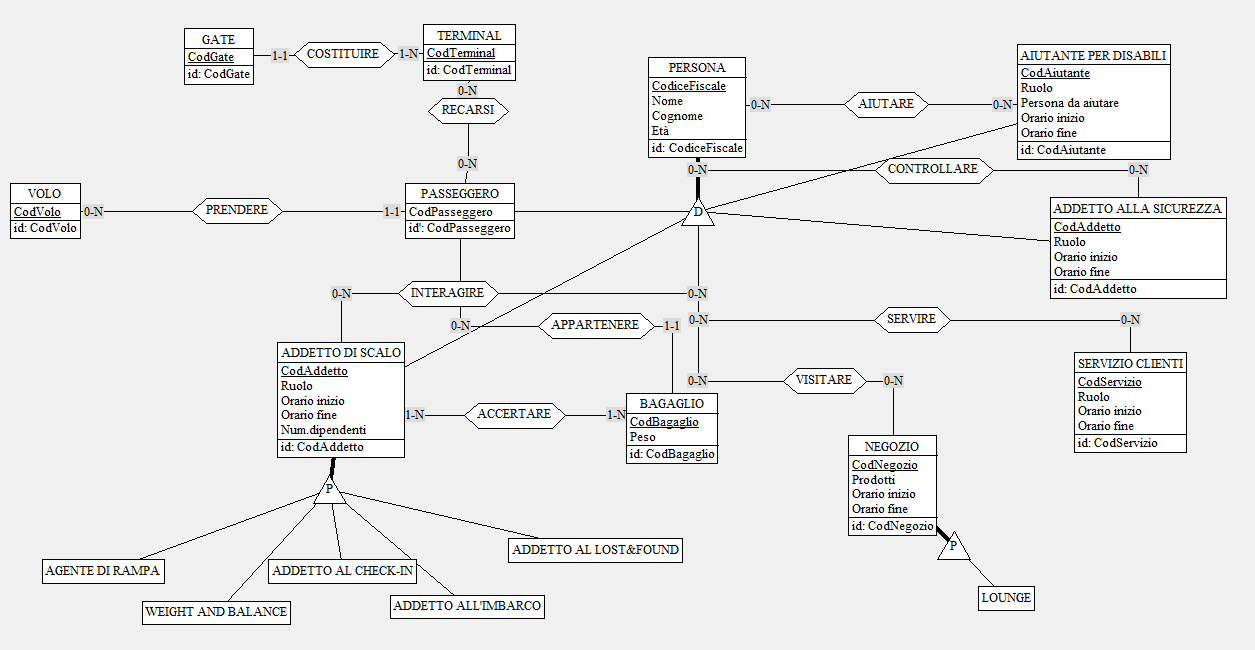
\includegraphics[width=1.2\textwidth, height=1.2\textheight, keepaspectratio]{./img/Schema_Concettuale/Passeggero.png}
	\caption{Schema concettuale di un Passeggero.}
	\label{fig:schema_passeggero}
\end{figure}

\pagebreak

\textsf{Un \textbf{passeggero} che è una figura centrale per il funzionamento di un Aeroporto, può avere diverse relazioni con le \textbf{persone} che lavorano al suo interno:}\\
%che è una figura importante per il funzionamento di un Aeroporto, può avere diverse relazioni con le varie \textbf{persone} che lavorano al suo interno.}

% qui prima era senza lista.
\begin{itemize}
	\item \textsf{\small \emph{Può essere controllato} dagli \textbf{addetti di scalo}, quali \textbf{addetti alla sicurezza} e \textbf{addetti al check-in} .}\\
	\item \textsf{\small \emph{Può visitare} i \textbf{negozi} e le \textbf{lounge} delle \textbf{compagnie aeree}}.\\
	\item \textsf{\small \emph{Può recarsi} al \textbf{servizio clienti} per ottenere informazioni e comprare i biglietti.}\\
	\item \textsf{\small \emph{Può}, una volta comprato un biglietto e superato i controlli \emph{recarsi} al \textbf{terminal} per poi giungere al \textbf{gate} per imbarcarsi e prendere un \textbf{volo}.}\\
\end{itemize}

%\textsf{\small Il \textbf{passeggero} , gli \textbf{Addetti di scalo}, \textbf{addetti alla sicurezza}, \textbf{aiutanti per disabili} sono una generalizzazione di una entità \textbf{persona}. }

% -------------- SCHEMA CONCETTUALE COMPAGNIA AEREA -----------------------------

\newpage

\subsubsection{Compagnia Aerea}

\textsf{\small Dopo aver analizzato il dominio, i problemi e le richieste della Compagnia Aerea, viene qui mostrato il suo schema parziale:}

\begin{figure}[H] 
	\centering
	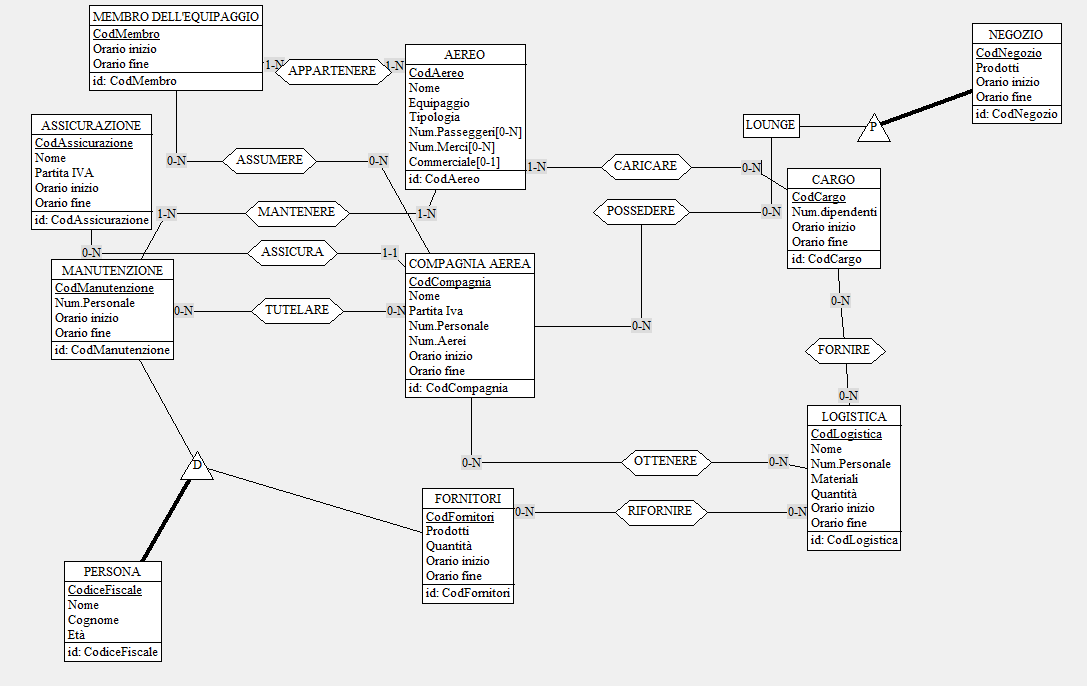
\includegraphics[width=1.2\linewidth, height=1.2\textheight, keepaspectratio]{./img/Schema_Concettuale/Compagnia_Aerea.png}
	\caption{Schema E/R della Compagnia Aerea.}
	\label{fig:schema_compagnia_aerea}
\end{figure}

\textsf{\small Le entità \textbf{Fornitori}, \textbf{Manutentori} e \textbf{Membro dell'equipaggio} rappresentano una estensione più generica di una entità \textbf{Persona}.  }\\

\textsf{\small Una \textbf{compagnia aerea} possiede diversi costi, uno dei primi è in gergo aeronautico \emph{ACMI}, ovvero \emph{Aircraft, Crew, Maintanance, Insurance} (in italiano: \textbf{Aereo}, \textbf{Equipaggio},\textbf{Manutenzione},\textbf{Assicurazione}).}\\

\textsf{\small Inoltre la Compagnia deve rifornire attraverso la \textbf{Logistica} ed il \textbf{Cargo} gli Aerei di beni necessari per il corretto funzionamento del Volo, come carburante, catering, cibo e bevande,ecc..}\\

% -------------- SCHEMA CONCETTUALE CONTROLLORE -----------------------------

\newpage

\enlargethispage{1\linewidth}

\subsubsection{Controllore}

\textsf{\small Figura centrale nella coordinazione e la sicurezza di navigazione degli aeromobili sono i \textbf{Controllori}: }\\
\begin{itemize}
	\item \textbf{\small Di Torre}
	\item \textbf{\small Di Avvicinamento}
	\item \textbf{\small D'Aerea}
\end{itemize}

\textsf{\small questi, rappresentano una estensione più generica di una entità \textbf{Persona}.}\\

\begin{figure}[H] 
	\centering
	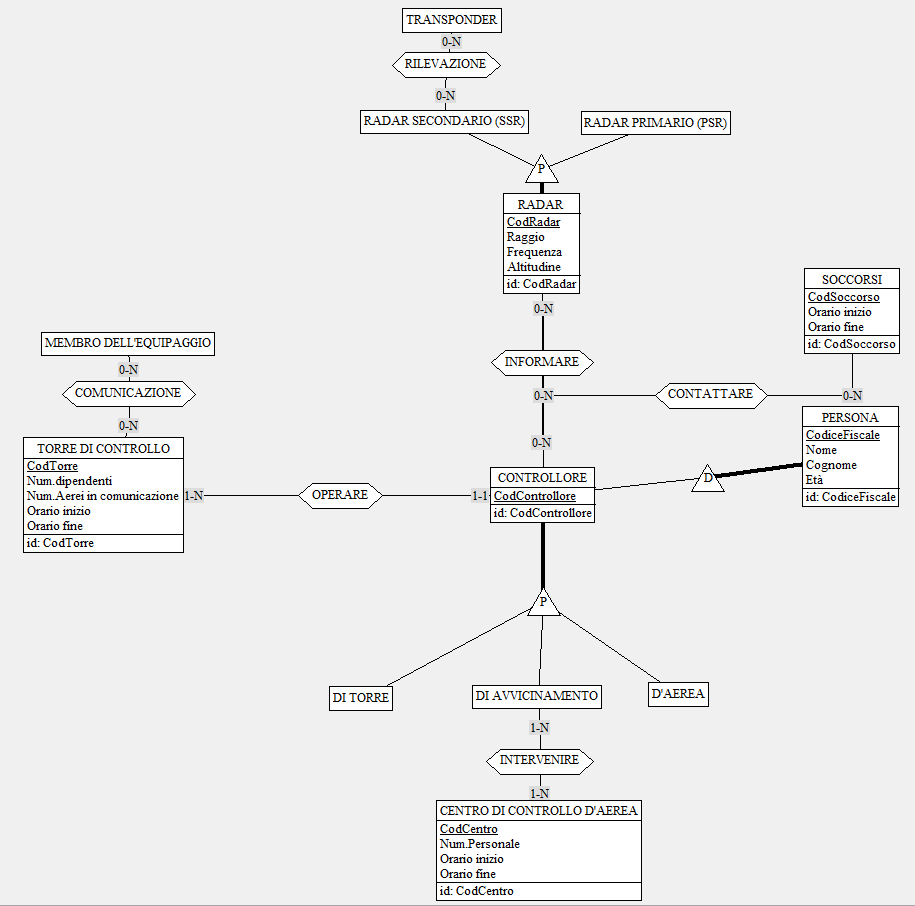
\includegraphics[width=1.2\linewidth, height=1.2\textheight, keepaspectratio]{./img/Schema_Concettuale/Controllore.png}
	\caption{Schema E/R di un Controllore del traffico aereo.}
	\label{fig:schema_controllore}
\end{figure}

\pagebreak

\textsf{\small I \textbf{Controllori}, nella \textbf{Torre di Controllo} o in un \textbf{Centro di Controllo d'Aerea}, attraverso l'utilizzo di uno strumento avanzato di localizzazione chiamato \textbf{Radar} comunicano, organizzano, coordinano il traffico aereo.}\break

% Questa parte è più tecnica che riguardante l'E/R, forse è meglio metterla
% nella parte di analisi/intervista.
\textsf{\small I \textbf{controllori} hanno a che fare con due principali tipi di radar, il PSR (\emph{Primary Surveillance Radar}), \textbf{radar primario di sorveglianza} che \emph{rileva} la posizione di un aeromobile analizzando i segnali che, precedentemente emessi dall'antenna, sono ritornati indietro riflessi dall'obiettivo; dopodichè la posizione dell'aereo può essere letta dall'operatore attraverso uno schermo su cui viene mostrata come una traccia luminosa.}\\

\textsf{\small E il SSR (\emph{Secondary Surveillance Radar}), \textbf{radar secondario di sorveglianza} che a differenza del primario, \emph{rileva} la posizione di un aeromobile analizzando il segnale trasmesso da un apparato a bordo dell'aeromobile (\emph{transponder}), emesso come risposta all'interrogazione ricevuta dal \textbf{radar} a terra.}\break

\textsf{\small In caso di emergenze (\emph{Mayday}), sono pronti a \emph{contattare} i \textbf{soccorsi} che dovranno prestare un tempestivo intervento per garantire la sicurezza dei passeggeri a bordo e del personale aeroportuale a terra. }\\

% -------------- SCHEMA CONCETTUALE VOLO -----------------------------

\newpage

\subsubsection{Volo}

%\textsf{\small Il \textbf{Volo}, l'origine per cui nasce l'Aeroporto, per la navigazione degli aeromobili è qui mostrato in questo ultimo schema parziale.}\\

\textsf{\small Esso congiunge il mezzo, l'\textbf{Aereo} e coloro che debbono usufruire del servizio, i \textbf{Passeggeri}.}\\

\begin{figure}[H] 
	\centering
	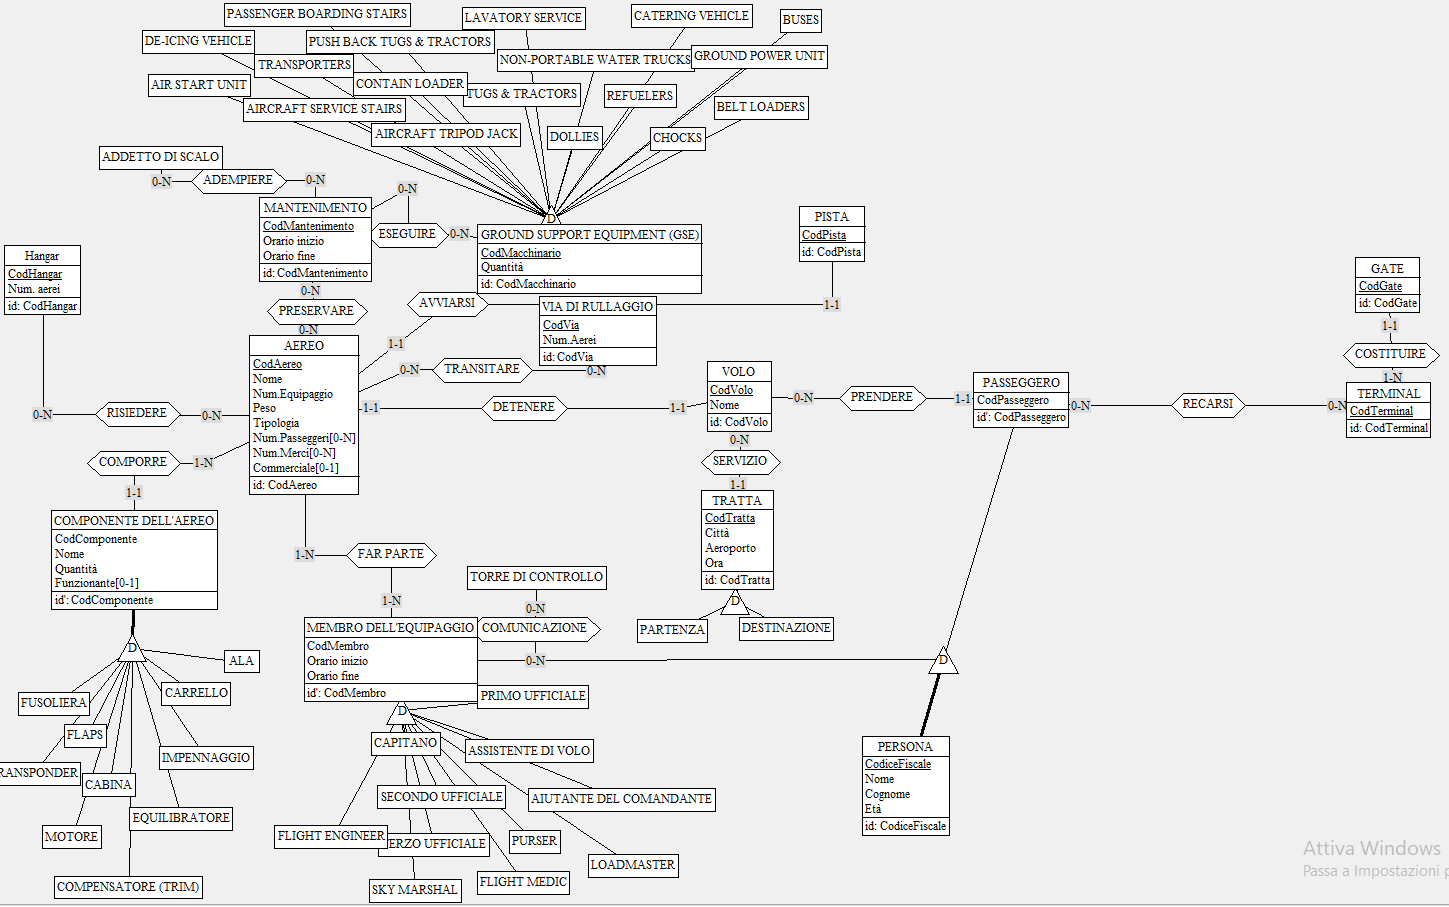
\includegraphics[width=1.2\linewidth, height=1.2\textheight, keepaspectratio]{./img/Schema_Concettuale/Volo.png}
	\caption{Schema E/R del Volo.}
	\label{fig:schema_volo}
\end{figure}

\textsf{\small Un \textbf{Volo} è formato da una \textbf{Tratta} ed un \textbf{Orario}.}\\

\textsf{\small Inoltre, un \textbf{Volo} deve mantenere il contatto radio con la \textbf{Torre di Controllo} per il coordinamento del traffico aereo.}\\

\textsf{\small Ogni \textbf{Aereo} è composto da questi principali componenti:}

\begin{itemize}
	\item \textbf{\small Fusoliera}
	\item \textbf{\small Flaps}
	\item \textbf{\small Ala}
	\item \textbf{\small Carrello}
	\item \textbf{\small Impennaggio}
	\item \textbf{\small Equilibratore}
	\item \textbf{\small Cabina}
	\item \textbf{\small Motore}
	\item \textbf{\small Transponder}
	\item \textbf{\small Compensatore (Trim)}
\end{itemize}

\textsf{\small ed è formato da questi membri dell'equipaggio:}

\textsf{\small \emph{Capitano, Primo Ufficiale, Secondo Ufficiale, Terzo Ufficiale, Flight Engineer, Sky Marshal, Flight Medic, Aiutante del Comandante, Assistente di Volo, Purser, Loadmaster}.} \break

\textsf{\small Di vitale importanza per lo svolgimento in sicurezza delle normali operazioni aeronautiche è la \textbf{Manutenzione}, sia degli \textbf{Addetti di scalo} sia del \textbf{Ground Support Equipment (GSE)}.}\\

\textsf{\small Il \textbf{GSE} è composto da: }\\

\textsf{\small \emph{ Dollies, Chocks, Aircraft Tripod Jack, Aircraft Service Stairs, Refuelers, Tugs and Tractors, Ground Power Unit, Buses, Contain Loader, Transporters, Air Start Unit, Non-portable Water Trucks, Lavatory Service Vehicles, Pushback tugs and tractors, De/anti-Icing Vehicle, Catering Vehicle, Belt Loaders, Passenger Boarding Steps, Aircraft Rescue and Firefighting}.}\\

% -------------- SCHEMA CONCETTUALE FINALE---------------------------------------

%\enlargethispage{1\linewidth}

\subsection{Schema concettuale finale}

\textsf{\small Dati i quattro schemi parziali inziali, presento ora lo \textbf{Schema Concettuale Finale}:}\\

% landscape


%\newgeometry{left = .9mm, right = .9mm, top = .9mm, bottom = .9mm} %TODO: o .6 o .9, top = .6, bottom = .6

\begin{comment}
\begin{sidewaysfigure}[H]
	\includegraphics[width=1.2\textwidth]{./img/Schema_Finale1.png} %TODO: 1 o 1.1 o 1.2, con 1.2 perdiamo delle informazioni, ma si vedo meglio
	\caption{}
	\label{fig:s1}
\end{sidewaysfigure}


\begin{sidewaysfigure}[H]
	\includegraphics[width=1.2\textwidth]{./img/Schema_Finale2.png}
	\caption{}
	\label{fig:s2}
\end{sidewaysfigure}

\begin{sidewaysfigure}[H]
	\includegraphics[width=1.2\textwidth]{./img/Schema_Finale3.png}
	\caption{}
	\label{fig:s3}
\end{sidewaysfigure}

\begin{sidewaysfigure}[H]
	\includegraphics[width=1.2\textwidth]{./img/Schema_Finale4.png}
	\caption{}
	\label{fig:s4}
\end{sidewaysfigure}
\end{comment}

%\restoregeometry

\begin{comment}
\begin{landscape}
	\begin{figure}[H]
		\centering
		\includegraphics[width=1.2\linewidth, height=1.2\textheight, keepaspectratio]{./img/Schema_Finale1.png}
		\caption{Schema concettuale Finale.}
		\label{fig:schema_finale}
	\end{figure}
\end{landscape}
\end{comment}

%TODO: sistemare
\newgeometry{left = .6cm, right = .6cm, top=.1cm, bottom=.1cm} % prima top = 5mm, bottom = 10mm

\begin{figure}[H] 
	\centering
	\includegraphics[width=1.2\linewidth, height=1.2\textheight, keepaspectratio]{./img/Schema_Concettuale/Schema_Finale1.png} 
	\caption{Schema concettuale Finale.}
	\label{fig:schema_finale1}
\end{figure}

\begin{figure}[H] 
	\centering
	\includegraphics[width=1.2\linewidth, height=1.2\textheight, keepaspectratio]{./img/Schema_Concettuale/Schema_Finale2.png}
	\caption{Schema concettuale Finale.}
	\label{fig:schema_finale2}
\end{figure}

\begin{figure}[H] 
	\centering
	\includegraphics[width=1.2\linewidth, height=1.2\textheight, keepaspectratio]{./img/Schema_Concettuale/Schema_Finale3.png}
	\caption{Schema concettuale Finale.}
	\label{fig:schema_finale3}
\end{figure}

\begin{figure}[H] 
	\centering
	\includegraphics[width=1.2\linewidth, height=1.2\textheight, keepaspectratio]{./img/Schema_Concettuale/Schema_Finale4.png}
	\caption{Schema concettuale Finale.}
	\label{fig:schema_finale4}
\end{figure}

\restoregeometry

\begin{comment}
\begin{landscape}
	\begin{figure}[H] %TODO: sistemare grandezza
		\centering
		\includegraphics[width=1\linewidth, height=1\textheight, keepaspectratio]{./img/Schema_Finale1.png} %TODO: o 1 o 1.3 o 1.2
		\caption{Schema concettuale Finale.}
		\label{fig:schema_finale44}
	\end{figure}
\end{landscape}
\end{comment}
	
	% --------------- PROGETTAZIONE LOGICA ------------------------------------------

\newpage

\section{Progettazione Logica} %TODO: riguardarsi tutta questa parte.

\subsection{Stima del volume di dati}

\begin{tabular}{ | c  c  c | c  c  c | } %TODO: sistemare, alcune vuote sono per separare, altre perchè manca. (aggiungere quelle che mancano)
	%TODO: aggiungere i numeri del volume.
	\hline
	\textbf{Concetto} & \textbf{Tipo} & \textbf{Volume} & \textbf{Concetto} & \textbf{Tipo} & \textbf{Volume}\\
	\hline
	\textsf{\small Passeggero} & \textsf{\small E} & \textsf{\small $ 200.000$} & \textsf{\small Aereo} & \textsf{\small E} & \textsf{\small $ $}\\
	\hline
	\textsf{\small Terminal} & \textsf{\small E} & \textsf{\small $ $} & \textsf{\small Membro dell'equipaggio} & \textsf{\small E} & \textsf{\small $ $}\\
	\hline
	\textsf{\small Recarsi} & \textsf{\small R} & \textsf{\small $ $} & \textsf{\small Pilotare} & \textsf{\small R} & \textsf{\small $ $}\\
	\hline
	\textsf{\small Negozio} & \textsf{\small E} & \textsf{\small $ $} & \textsf{\small Pista} & \textsf{\small E} & \textsf{\small $ $}\\
	\hline
	\textsf{\small Comprare} & \textsf{\small R} & \textsf{\small $ $} & \textsf{\small Avvio} & \textsf{\small R} & \textsf{\small $ $}\\
	\hline
	\textsf{\small Addetto di Scalo} & \textsf{\small E} & \textsf{\small $ $} & \textsf{\small Via di rullaggio} & \textsf{\small E} & \textsf{\small $ $}\\
	\hline
	\textsf{\small Interagire} & \textsf{\small R} & \textsf{\small $ $} & \textsf{\small Ground Support Equipment} & \textsf{\small E} & \textsf{\small $ $}\\
	\hline
	\textsf{\small Addetto alla sicurezza} & \textsf{\small E} & \textsf{\small $ $} & \textsf{\small Eseguita} & \textsf{\small R} & \textsf{\small $ $}\\
	\hline
	\textsf{\small Controllare} & \textsf{\small R} & \textsf{\small $ $} & \textsf{\small } & \textsf{\small } & \textsf{\small $ $}\\
	\hline
	\textsf{\small Aiutante per disabili} & \textsf{\small E} & \textsf{\small $ $} & \textsf{\small } & \textsf{\small } & \textsf{\small $ $}\\
	\hline
	\textsf{\small Aiutare} & \textsf{\small R} & \textsf{\small $ $} & \textsf{\small } & \textsf{\small } & \textsf{\small $ $}\\
	\hline
	\textsf{\small Volo} & \textsf{\small E} & \textsf{\small $ $} & \textsf{\small } & \textsf{\small } & \textsf{\small $ $}\\
	\hline
	\textsf{\small Volare} & \textsf{\small R} & \textsf{\small $ $} & \textsf{\small } & \textsf{\small } & \textsf{\small $ $}\\
	\hline
	\textsf{\small } & \textsf{\small } & \textsf{\small $ $} & \textsf{\small } & \textsf{\small } & \textsf{\small $ $} \\
	\hline
	\textsf{\small Controllore} & \textsf{\small E} & \textsf{\small $ $} & \textsf{\small } & \textsf{\small } & \textsf{\small $ $}\\
	\hline
	\textsf{\small Controllo} & \textsf{\small R} & \textsf{\small $ $} & \textsf{\small } & \textsf{\small } & \textsf{\small $ $}\\
	\hline
	\textsf{\small Torre di Controllo} & \textsf{\small E} & \textsf{\small $ $} & \textsf{\small } & \textsf{\small } & \textsf{\small $ $}\\
	\hline
	\textsf{\small Radar} & \textsf{\small E} & \textsf{\small $ $} & \textsf{\small } & \textsf{\small } & \textsf{\small $ $}\\
	\hline
	\textsf{\small Informare} & \textsf{\small R} & \textsf{\small $ $} & \textsf{\small } & \textsf{\small } & \textsf{\small $ $}\\
	\hline
	\textsf{\small Comunicazione} & \textsf{\small R} & \textsf{\small $ $} & \textsf{\small } & \textsf{\small } & \textsf{\small $ $}\\
	\hline
	\textsf{\small Rilevazione} & \textsf{\small R} & \textsf{\small $ $} & \textsf{\small } & \textsf{\small } & \textsf{\small $ $}\\
	\hline
	\textsf{\small } & \textsf{\small } & \textsf{\small $ $} & \textsf{\small } & \textsf{\small } & \textsf{\small $ $}\\
	\hline
	\textsf{\small Compagnia Aerea} & \textsf{\small E} & \textsf{\small $ $} & \textsf{\small } & \textsf{\small } & \textsf{\small $ $}\\
	\hline
	\textsf{\small Manutenzione} & \textsf{\small E} & \textsf{\small $ $} & \textsf{\small } & \textsf{\small } & \textsf{\small $ $}\\
	\hline
	\textsf{\small } & \textsf{\small } & \textsf{\small $ $} & \textsf{\small } & \textsf{\small } & \textsf{\small $ $}\\
	\hline
	\textsf{\small Fornitori} & \textsf{\small E} & \textsf{\small $ $} & \textsf{\small } & \textsf{\small } & \textsf{\small $ $}\\
	\hline
	\textsf{\small Rifornire} & \textsf{\small R} & \textsf{\small $ $} & \textsf{\small } & \textsf{\small } & \textsf{\small $ $}\\
	\hline
	\textsf{\small Logistica} & \textsf{\small E} & \textsf{\small $ $} & \textsf{\small } & \textsf{\small } & \textsf{\small $ $}\\
	\hline
	\textsf{\small Cargo} & \textsf{\small E} & \textsf{\small $ $} & \textsf{\small } & \textsf{\small } & \textsf{\small $ $}\\
	\hline
	\textsf{\small Fornire} & \textsf{\small R} & \textsf{\small $ $} & \textsf{\small } & \textsf{\small } & \textsf{\small $ $}\\
	\hline
	\textsf{\small Mantenere} & \textsf{\small R} & \textsf{\small $ $} & \textsf{\small } & \textsf{\small } & \textsf{\small $ $}\\
	\hline
	\textsf{\small Caricare} & \textsf{\small R} & \textsf{\small $ $} & \textsf{\small } & \textsf{\small } & \textsf{\small $ $}\\
	\hline
	\textsf{\small Possedere} & \textsf{\small R} & \textsf{\small $ $} & \textsf{\small } & \textsf{\small } & \textsf{\small $ $}\\
	\hline
\end{tabular}

% ---- DESCRIZIONE DELLE OPERAZIONI PRINCIPALI E STIMA DELLA LORO FREQUENZA -----

\newpage

\subsection{Descrizione delle operazioni principale e stima della loro frequenza}

%TODO: modificare alcune operazioni per, per esempio, trovare non so, quanti dipendenti hanno età > 20; oppure quanti litri di carburante sono rimasti all'aereo.

\textsf{\small Si fornisce, di seguito, una tabella riportante la descrizione e la relativa frequenza delle operazioni principali nell'Aeroporto.}\\

\begin{tabular}{ | c c c |} %TODO: aggiungere operazioni mancanti
	\hline
	\textbf{Codice} & \textbf{Operazione} & \textbf{Frequenza} \\
	\hline
	\textsf{\small 01} & \textsf{\small Registrare un nuovo passeggero} & \textsf{\small $5000/\text{giorno}$} \\ % 200.000 / 30 = 6666.6 (-1000)
	\hline
	\textsf{\small 02} & \textsf{\small  Numero totale di componenti non funzionanti in un aereo.} & \textsf{\small $  $} \\ %TODO: aggiungere
	\hline
	\textsf{\small 03} & \textsf{\small Voli in partenza} & \textsf{\small $ 1000 / \text{mese} $} \\
	% Voli in partenza:
	% Ho preso la media del numero dei passeggeri che un aereo può portare
	% da questo sito (che mostra gli aerei più comuni) https://www.ponderweasel.com/how-many-people-can-fit-on-a-plane/?__cf_chl_managed_tk__=pmd_2mLayow7P2xTK3G5HcerVGqTNeA1cnsOiQfUmRb1Vok-1635365141-0-gqNtZGzNAxCjcnBszQh9
	% escludendo gli aerei privati e da singoli ed ho ottenuto:
	% una media pari a 
	% 525 + 220 + 189 + 290 + 451 + 366 + 172 / 7 = 316,14 -> 316
	% Se io ho scritto 5000 passeggeri / giorno, allora
	% 5000 / 316 = 15.82 -> 16 aerei per trasportare queste 5000 persone ogni giorno
	% in un mese 16 * 31 = 496 però tenendo conto che questa è una media così
	% e non tutti gli aerei possono portare tanto quanto il numero medio allora
	% metto 1000.
	\hline
	\textsf{\small 04} & \textsf{\small Voli in arrivo} & \textsf{\small $ 1000 / \text{mese} $} \\
	\hline
	\textsf{\small 05} & \textsf{\small Manutenzione di un aereo} & \textsf{\small $ 2000 / \text{mese} $} \\
	\hline
	\textsf{\small 06} & \textsf{\small Comunicazioni tra controllori e membri dell'equipaggio di un aereo} & \textsf{\small $ 1000 / \text{giorno} $} \\
	% [3 (departure) + 3 (arrival) + 3 + 3 + (eventuali emergenze) ] * (2000 / 30) = 800 / comunicazioni al giorno. oppure 15 * (2000 / 30) = 1000
	
	% oppure
	
	% 238 persone circa per aeroplano, 238 * 840 = 199.920 passeggeri
	% 840 voli / 30 giorni = 28 / voli al giorno
	
	% oppure
	
	% 130 passeggeri per volo.
	% 130 * 1540 = 200.200 passeggeri
	% 1540 voli / 30 giorni = 51 / voli giornalieri
	
	\hline
	\textsf{\small 07} & \textsf{\small Rifornimento di un aereo} & \textsf{\small $ 2000/ \text{mese} $} \\
	\hline
	\textsf{\small 08} & \textsf{\small Assunzione di nuovi addetti} & \textsf{\small $ 1000 / \text{anno}$} \\
	\hline
	\textsf{\small 09} & \textsf{\small Operazioni di check-in} & \textsf{\small $ 5000 / \text{giorno}$} \\
	\hline
	\textsf{\small 10} & \textsf{\small Aerei in pista} & \textsf{\small $ 2000 / \text{mese}$} \\
	\hline
	\textsf{\small 11} & \textsf{\small Persone che comprano prodotti ai negozi} & \textsf{\small $ 1000 / \text{giorno} $} \\ %TODO: Scrivere Acquirenti ai negozi? però non ho un'entità Acquirente.
	% Persone != Passeggeri e quindi le persone potrebbero essere di più dei passeggeri, però non tuti vanno per i negozi e ancora di meno sono quelli che comprano. Quindi quelli che visitano i negozi diciamo che sono 2000/giorno, ma quelli che comprano sono diciamo circa 1000/giorno o anche meno, magari 500.
	\hline
	\textsf{\small 12} & \textsf{\small Persone che si recano al Terminal} & \textsf{\small $ 5000 / \text{giorno} $} \\
	\hline
	\textsf{\small 13} & \textsf{\small Nuovi membri dell'equipaggio assunti da una compagnia} & \textsf{\small $ 500 / \text{anno}$} \\ %TODO: se gli addetti sono 1000 all'anno, questi saranno un po' di meno, immagino, diventare piloti richiede tempo.
	\hline
	\textsf{\small 14} & \textsf{\small Inserimento di aerei stazionati negli hangar} & \textsf{\small $ 500 / \text{mese} $} \\ % (Quite big) Boeing 747 : 5600 square feet, quite big hangar : 317000 square feet.
	% 317000 / 5600 = 56,6 -> 57
	% Gli hangar sono più di uno.
	\hline
	\textsf{\small 15} & \textsf{\small Calcolare l'età media dei passeggeri} & \textsf{\small $ 1 / \text{mese} $} \\
	\hline
	\textsf{\small 16} & \textsf{\small Ottenere il numero di aerei di una compagnia aerea.} & \textsf{\small $ 1 / \text{anno} $} \\
	\hline
	\textsf{\small 17} & \textsf{\small Numero di controllori in una Torre di Controllo} & \textsf{\small $ 1 / \text{anno} $} \\
	\hline
	\textsf{\small 18} & \textsf{\small Numero di macchinari presenti nell'Aeroporto} & \textsf{\small $ 1 / \text{mese} $} \\
	\hline
	\textsf{\small 19} & \textsf{\small Approvvigionamento dell'aereo} & \textsf{\small $ 2000 / \text{mese} $} \\
	% L'aeroporto compra il carburante e poi lo vende alle compagnie aeree.
	% altre risorse possono essere di cibo, di acqua, di servizi di catering,ecc..
	\hline
	\textsf{\small 20} & \textsf{\small Numero aerei commerciali di una compagnia aerea} & \textsf{\small $ 1/ \text{mese} $} \\
	\hline
	\textsf{\small 21} & \textsf{\small Quantità di merci trasportate in media da un aereo commerciale} & \textsf{\small $ 1/ \text{mese} $} \\
	\hline
	%TODO: add Numero di aerei di linea di una compagnia aerea ?
\end{tabular}

% ----- SCHEMI DI NAVIGAZIONE E TABELLE DEGLI ACCESSI --------------------------

%TODO: ragionarla in termini di SQL. Per questo serviranno accedere ad altre relazioni,ecc...

\newpage

\subsection{Schemi di navigazione e tabelle degli accessi}

\textsf{\small Dopo aver stimato il volume dei dati ed elencato le principali operazioni, vengono riportati qui i loro relativi schemi di navigazione. \emph{Si considerino di doppio peso gli accessi in scrittura rispetto a quelli in lettura}.}\break


%TODO: sistemare le varie opzioni e ricontrollare se basta una sola scrittura/lettura o servono di più.

% OP 1 | Registrare un nuovo passeggero

\textbf{\small OP 1 | Registrare un nuovo passeggero}\\

\begin{tabular}{ c c c c}
	%\textbf{\small OP 1 | Registrare un nuovo passeggero} & & & \\
	\hline
	\textbf{Concetto} & \textbf{Costrutto} & \textbf{Accesi} & \textbf{Tipo}\\
	\hline
	\textsf{\small Passeggero} & \textsf{\small E} & \textsf{\small 1} &  \textsf{\small S}\\
	\hline
	\textsf{\small } & \textsf{\small } & \textbf{Totale: 1S $\rightarrow 10000$/giorno} \textsf{\small } & \textsf{\small }\\ % 2 * 5000/giorno = 10000/giorno
	\hline
\end{tabular}

\vspace{.6cm}

% OP 2 | Numero totale di componenti non funzionanti in un aereo.

\textbf{\small OP 2 | Numero totale di componenti non funzionanti in un aereo.}\\
%TODO: fix
%\textsf{\small Tra le migliaia di persone giornaliere, non vengono necessariamente controllate tutte, ma solo quelle di cui si ha dei sospetti o si vogliono fare ulteriori accertamenti. (con controllo non intendo il check-in).}\break

\begin{tabular}{ c c c c} %TODO: aggiungere le altre entitò e relazioni per il controllo di un passeggero
	%\textbf{\small OP 2 | Controllare un passeggero} & & & \\
	\hline
	\textbf{Concetto} & \textbf{Costrutto} & \textbf{Accesi} & \textbf{Tipo}\\
	\hline
	\textsf{\small R} & \textsf{\small Controllare} & \textsf{\small 1} &  \textsf{\small L}\\
	\hline
	\textsf{\small } & \textsf{\small } & \textbf{Totale: 1L $\rightarrow 1000$/giorno} \textsf{\small } & \textsf{\small }\\ % non si controllano mica tutte le persone, solo alcune di cui si ha dei sospetti o si vogliono fare ulteriori accertamenti.
	\hline
\end{tabular}

\vspace{.6cm}

% OP 3 | Voli in partenza

\textbf{\small OP 3 | Voli in partenza}\\

\begin{tabular}{ c c c c} %TODO: aggiungere TRATTA
	%\textbf{\small OP 3 | Voli in partenza} & & & \\
	\hline
	\textbf{Concetto} & \textbf{Costrutto} & \textbf{Accesi} & \textbf{Tipo}\\
	\hline
	\textsf{\small E} & \textsf{\small Partenza (Tratta)} & \textsf{\small 1} &  \textsf{\small S}\\
	\hline
	\textsf{\small } & \textsf{\small } & \textbf{Totale: 1S $\rightarrow 2000$/mese} \textsf{\small } & \textsf{\small }\\
	\hline
\end{tabular}

\vspace{.6cm}

% OP 4 | Voli in arrivo

\textbf{\small OP 4 | Voli in arrivo}\\

\begin{tabular}{ c c c c} %TODO: aggiungere TRATTA e VOLO
	%\textbf{\small OP 4 | Voli in arrivo} & & & \\
	\hline
	\textbf{Concetto} & \textbf{Costrutto} & \textbf{Accesi} & \textbf{Tipo}\\
	\hline
	\textsf{\small E} & \textsf{\small Destinazione (Tratta)} & \textsf{\small 1} &  \textsf{\small S}\\
	\hline
	\textsf{\small } & \textsf{\small } & \textbf{Totale: 1S $\rightarrow 2000$/mese } \textsf{\small } & \textsf{\small }\\
	\hline
\end{tabular}

\vspace{.6cm}

% OP 5 | Manutenzione di un aereo

\textbf{\small OP 5 | Manutenzione di un aereo}\\

\begin{tabular}{ c c c c} %TODO: aggiungere aereo?
	%\textbf{\small OP 5 | Manutenzione di un aereo} & & & \\
	\hline
	\textbf{Concetto} & \textbf{Costrutto} & \textbf{Accesi} & \textbf{Tipo}\\
	\hline
	\textsf{\small E} & \textsf{\small Manutenzione} & \textsf{\small 1} &  \textsf{\small S}\\
	\hline
	\textsf{\small } & \textsf{\small } & \textbf{Totale: 1S $\rightarrow 4000$/mese} \textsf{\small } & \textsf{\small }\\
	\hline
\end{tabular}

\vspace{.6cm}

% OP 6 | Comunicazioni tra controllori e membri dell'equipaggio di un aereo

\textbf{\small OP 6 | Comunicazioni tra controllori e membri dell'equipaggio di un aereo}\\

\begin{tabular}{ c c c c} %TODO: aggiungere Torre di Controllo, Controllore ed membro dell'equipaggio (non membro, ma VOLO e magari AEREO)
	%\textbf{\small OP 6 | Comunicazioni tra controllori e membri dell'equipaggio di un aereo} & & & \\
	\hline
	\textbf{Concetto} & \textbf{Costrutto} & \textbf{Accesi} & \textbf{Tipo}\\
	\hline
	\textsf{\small R} & \textsf{\small Comunicazione (Torre di Controllo)} & \textsf{\small 1} &  \textsf{\small S}\\
	\hline
	\textsf{\small } & \textsf{\small } & \textbf{Totale: 1S$\rightarrow 2000$/giorno } \textsf{\small } & \textsf{\small }\\
	\hline
\end{tabular}

\vspace{.6cm}

% OP 7 | Rifornimento di un aereo

%TODO: dalla 7 alla 14, scrivere qualche cosa.

\newpage %\pagebreak

\textbf{\small OP 7 | Rifornimento di un aereo}\\

\begin{tabular}{ c c c c}
	%\textbf{\small OP 7 | } & & & \\
	\hline
	\textbf{Concetto} & \textbf{Costrutto} & \textbf{Accesi} & \textbf{Tipo}\\
	\hline
	\textsf{\small E} & \textsf{\small GSE} & \textsf{\small 1} &  \textsf{\small S}\\
	\hline
	\textsf{\small } & \textsf{\small } & \textbf{Totale: 1S$\rightarrow 4000$/mese } \textsf{\small } & \textsf{\small }\\
	\hline
\end{tabular}

\vspace{.6cm}

% OP 8 | Assunzione di nuovi addetti

\textbf{\small OP 8 | Assunzione di nuovi addetti}\\

\begin{tabular}{ c c c c}
	%\textbf{\small OP 8 | } & & & \\
	\hline
	\textbf{Concetto} & \textbf{Costrutto} & \textbf{Accesi} & \textbf{Tipo}\\
	\hline
	\textsf{\small E} & \textsf{\small Addetto di Scalo} & \textsf{\small 1} &  \textsf{\small L}\\ %TODO: prima avevo messo lettura, ma un nuovo addetto mi sembra sia più una scrittura che una lettura
	\hline
	\textsf{\small } & \textsf{\small } & \textbf{Totale: 1S$\rightarrow 2000$/anno } \textsf{\small } & \textsf{\small }\\ % 2 * 1000 = 2000
	\hline
\end{tabular}

\vspace{.6cm}

% OP 9 | 

\textbf{\small OP 9 | Operazioni di check-in }\\

\begin{tabular}{ c c c c} %TODO: Aggiungere Addetto di Scalo.
	%\textbf{\small OP 9 | } & & & \\
	\hline
	\textbf{Concetto} & \textbf{Costrutto} & \textbf{Accesi} & \textbf{Tipo}\\
	\hline
	\textsf{\small R} & \textsf{\small Interagire} & \textsf{\small 1} &  \textsf{\small L}\\
	\hline
	\textsf{\small } & \textsf{\small } & \textbf{Totale: 1L$\rightarrow 5000$/giorno } \textsf{\small } & \textsf{\small }\\
	\hline
\end{tabular}

\vspace{.6cm}

% OP 10 | 

\textbf{\small OP 10 | Aerei in pista}\\

\begin{tabular}{ c c c c} %TODO: Aggiungere Aereo e relazione con pista
	%\textbf{\small OP 10 | } & & & \\
	\hline
	\textbf{Concetto} & \textbf{Costrutto} & \textbf{Accesi} & \textbf{Tipo}\\
	\hline
	\textsf{\small E} & \textsf{\small Pista} & \textsf{\small 1} &  \textsf{\small L}\\
	\hline
	\textsf{\small } & \textsf{\small } & \textbf{Totale: 1L$\rightarrow 2000$/mese } \textsf{\small } & \textsf{\small }\\
	\hline
\end{tabular}

\vspace{.6cm}

% OP 11 | Acquirenti ai negozi

\textbf{\small OP 11 | Acquirenti ai negozi}\\ %TODO: rimettere Persone che comprano prodotti ai negozi (o nei negozi).

\begin{tabular}{ c c c c}
	%\textbf{\small OP 11 | } & & & \\
	\hline
	\textbf{Concetto} & \textbf{Costrutto} & \textbf{Accesi} & \textbf{Tipo}\\
	\hline
	\textsf{\small E} & \textsf{\small Negozio} & \textsf{\small 1} &  \textsf{\small L}\\
	\hline
	\textsf{\small } & \textsf{\small } & \textbf{Totale: 1L$\rightarrow 1000$/giorno } \textsf{\small } & \textsf{\small }\\
	\hline
\end{tabular}

\vspace{.6cm}

% OP 12 | Passeggeri che si recano al Terminal
%TODO: meglio Persone o Passeggeri, teoricamente è più corretto Passeggeri.

\textbf{\small OP 12 | Persone che si recano al Terminal}\\

\begin{tabular}{ c c c c} %TODO: aggiungere Terminal
	%\textbf{\small OP 12 | } & & & \\
	\hline
	\textbf{Concetto} & \textbf{Costrutto} & \textbf{Accesi} & \textbf{Tipo}\\
	\hline
	\textsf{\small R} & \textsf{\small Recarsi} & \textsf{\small 1} &  \textsf{\small S}\\
	\hline
	\textsf{\small } & \textsf{\small } & \textbf{Totale: 1S$\rightarrow 10000$/giorno } \textsf{\small } & \textsf{\small }\\ % 2 * 5000 = 10000
	\hline
\end{tabular}

\vspace{.6cm}

% OP 13 | Nuovi membri dell'equipaggio assunti da una compagnia

\textbf{\small OP 13 | Nuovi membri dell'equipaggio assunti da una compagnia}\\

\begin{tabular}{ c c c c} %TODO: Aggiungere relazione Assumere e Membro dell'equipaggio.
	%\textbf{\small OP 13 | } & & & \\
	\hline
	\textbf{Concetto} & \textbf{Costrutto} & \textbf{Accesi} & \textbf{Tipo}\\
	\hline
	\textsf{\small E} & \textsf{\small Compagnia aerea} & \textsf{\small 1} &  \textsf{\small S}\\
	\hline
	\textsf{\small } & \textsf{\small } & \textbf{Totale: 1S$\rightarrow 1000$/anno } \textsf{\small } & \textsf{\small }\\ % 2 * 500 = 1000
	\hline
\end{tabular}

\vspace{.6cm}

% OP 14  | Inserimento di aerei stazionati negli Hangar

\textbf{\small OP 14 | Inserimento di aerei stazionati negli Hangar}\\

\begin{tabular}{ c c c c}
	%\textbf{\small OP 14 | } & & & \\
	\hline
	\textbf{Concetto} & \textbf{Costrutto} & \textbf{Accesi} & \textbf{Tipo}\\
	\hline
	\textsf{\small E} & \textsf{\small Hangar} & \textsf{\small 1} &  \textsf{\small S}\\
	\hline
	\textsf{\small } & \textsf{\small } & \textbf{Totale: 1S$\rightarrow 1000$/mese } \textsf{\small } & \textsf{\small }\\ % 2 * 500 == 1000
	\hline
\end{tabular}

\vspace{.6cm}

% OP 15 | Calcolare l'età media dei passeggeri

\textbf{\small OP 15 | Calcolare l'età media dei passeggeri}\\

\textsf{\small Ai fini statistici, per capire quali persone viaggiano di più, a che età e dove, ecc.. Viene registrata e calcolata l'età media delle persone e vari altri dati.}\break

\begin{tabular}{ c c c c}
	%\textbf{\small OP 15 | } & & & \\
	\hline
	\textbf{Concetto} & \textbf{Costrutto} & \textbf{Accesi} & \textbf{Tipo}\\
	\hline
	\textsf{\small E} & \textsf{\small Passeggero} & \textsf{\small 1} &  \textsf{\small L}\\
	\hline
	\textsf{\small E} & \textsf{\small Passeggero} & \textsf{\small 1} &  \textsf{\small S}\\ %TODO: per la scrittura della media.
	\hline
	\textsf{\small } & \textsf{\small } & \textbf{Totale: 1L + 1S$\rightarrow 2$/mese } \textsf{\small } & \textsf{\small }\\
	\hline
\end{tabular}

\vspace{.6cm}

% OP 16  | Ottenere il numero di aerei di una compagnia aerea

\textbf{\small OP 16 | Ottenere il numero di aerei di una compagnia aerea}\\

\begin{tabular}{ c c c c}
	%\textbf{\small OP 16 | } & & & \\
	\hline
	\textbf{Concetto} & \textbf{Costrutto} & \textbf{Accesi} & \textbf{Tipo}\\
	\hline
	\textsf{\small E} & \textsf{\small Compagnia Aerea} & \textsf{\small 1} &  \textsf{\small L}\\
	\hline
	\textsf{\small } & \textsf{\small } & \textbf{Totale: $\rightarrow $/ } \textsf{\small } & \textsf{\small }\\
	\hline
\end{tabular}

\vspace{.6cm}

% OP 17  | Numero di controllori in una Torre di Controllo

\textbf{\small OP 17 | Numero di controllori in una Torre di Controllo}\\

\begin{tabular}{ c c c c}
	%\textbf{\small OP 17 | } & & & \\
	\hline
	\textbf{Concetto} & \textbf{Costrutto} & \textbf{Accesi} & \textbf{Tipo}\\
	\hline
	\textsf{\small E} & \textsf{\small Torre di Controllo} & \textsf{\small 1} &  \textsf{\small L}\\
	\hline
	\textsf{\small } & \textsf{\small } & \textbf{Totale: 1L$\rightarrow 1$/anno } \textsf{\small } & \textsf{\small }\\
	\hline
\end{tabular}

\vspace{.6cm}

% OP 18  | Numero di macchinari presenti nell'Aeroporto

\textbf{\small OP 18 | Numero di macchinari presenti nell'Aeroporto}\\

\textsf{\small Per il controllo,la manutenzione dei vari macchinari e per la corretta esecuzione delle normali attività aeroportuali.}\break

\begin{tabular}{ c c c c}
	%\textbf{\small OP 18 | } & & & \\
	\hline
	\textbf{Concetto} & \textbf{Costrutto} & \textbf{Accesi} & \textbf{Tipo}\\
	\hline
	\textsf{\small E} & \textsf{\small GSE} & \textsf{\small 1} &  \textsf{\small L}\\
	\hline
	\textsf{\small } & \textsf{\small } & \textbf{Totale: 1L$\rightarrow 1$/mese } \textsf{\small } & \textsf{\small }\\
	\hline
\end{tabular}

\vspace{.6cm}

% OP 19  | Approvvigionamento dell'aereo

\textbf{\small OP 19 | Approvvigionamento dell'aereo}\\

\textsf{\small Rifornire l'aereo di varie risorse di primaria importanza per il suo funzionamento, non soltanto del carburante, ma anche di cibo, acqua, servizi di catering,ecc.. per il normale svolgimento delle operazioni e per il soddisfacimento dei bisogni dei passeggeri.}\break

\begin{tabular}{ c c c c}
	%\textbf{\small OP 19 | } & & & \\
	\hline
	\textbf{Concetto} & \textbf{Costrutto} & \textbf{Accesi} & \textbf{Tipo}\\
	\hline
	\textsf{\small E} & \textsf{\small GSE} & \textsf{\small 1} &  \textsf{\small S}\\
	\hline
	\textsf{\small } & \textsf{\small } & \textbf{Totale: 1S$\rightarrow 4000$/ mese} \textsf{\small } & \textsf{\small }\\
	\hline
\end{tabular}

\vspace{.6cm}

% OP 20  | Numero aerei commerciali di una compagnia aerea

\textbf{\small OP 20 | Numero aerei commerciali di una compagnia aerea}\\

\begin{tabular}{ c c c c}
	%\textbf{\small OP 20 | } & & & \\
	\hline
	\textbf{Concetto} & \textbf{Costrutto} & \textbf{Accesi} & \textbf{Tipo}\\
	\hline
	\textsf{\small E} & \textsf{\small Compagnia Aerea} & \textsf{\small 1} &  \textsf{\small L}\\
	\hline
	\textsf{\small } & \textsf{\small } & \textbf{Totale: 1L$\rightarrow 1$/mese } \textsf{\small } & \textsf{\small }\\
	\hline
\end{tabular}

\vspace{.6cm}

% OP 21  | Quantità di merci trasportate in media da un aereo commerciale

\textbf{\small OP 21 | Quantità di merci trasportate in media da un aereo commerciale}\\

\textsf{\small Per tenere traccia di quante merci sono state vendute e trasportate da una compagnia aerea.}\break

\begin{tabular}{ c c c c}
	%\textbf{\small OP 21 | } & & & \\
	\hline
	\textbf{Concetto} & \textbf{Costrutto} & \textbf{Accesi} & \textbf{Tipo}\\
	\hline
	\textsf{\small E} & \textsf{\small Compagnia Aerea} & \textsf{\small 1} &  \textsf{\small L}\\
	\hline
	\textsf{\small } & \textsf{\small } & \textbf{Totale: 1L$\rightarrow 1$/mese } \textsf{\small } & \textsf{\small }\\
	\hline
\end{tabular}

% --------------- RAFFINAMENTO DELLO SCHEMA ------------------------------------

\newpage

\subsection{Raffinamento dello schema}

%\subsubsection{Eliminazione gerarchie}
\textbf{Eliminazione delle gerarchie}\\
%TODO: quel superflue è corretto metterlo? o sarebbe da mettere nelle Ridondanze?
\textsf{\small Per quanto riguarda l'eliminazione delle gerarchie, ho deciso di adottare il collasso verso l'alto per la maggior parte di esse, come soluzione del problema, mentre per altre il collasso verso il basso.}\break 

% Collasso verso l'alto: Accorpare le entità figlie nel genitore

% Collasso verso il basso: Accorpare il genitore nelle entità figlie

\textsf{\small Ho individuato 8 gerarchie che ho collassato verso l'alto e aggiunto loro gli attributi \emph{Tipologia} o \emph{Ruolo}, ovvero \emph{Componente dell'aereo}, \emph{Membro dell'equipaggio}, \emph{Radar}, \emph{Controllore}, \emph{Addetto di scalo}, \emph{Negozio}, \emph{Ground Support Equipment},\emph{Tratta}.}\\

%TODO: Verso l'alto anche per Persona.
%TODO: Verso il basso solo per Terminal
\textsf{\small Per quanto riguarda \emph{Persona} invece ho ritenuto più opportuno adottare il collasso verso il basso, in quanto gli accessi alle entità figlie sono distinti.}\break
%TODO: collasso verso l'alto anche per Persona?

%TODO: metterlo nei ridondanti?

\textbf{Eliminazione degli attributi compositi}

\textsf{\small Non è stato fatto uso di attributi composti perciò non è stato dovuto assestare in alcun modo la faccenda.}\break %assestato, situazione/contesto.

\textbf{Scelte delle chiavi primarie}

\textsf{\small Nello schema proposto sono già presenti le chiavi primarie per tutte le entità, identificate ciascuna da un proprio codice univoco.}\break

\textbf{Eliminazione degli identificatori esterni}

\textsf{\small A seguito delle analisi compiute è stato determinato di rimuovere le seguenti relazioni:}\\ %deciso

% SOLO RELAZIONI
\begin{itemize} %TODO: forse alcune sono superflue, perchè le ho già cambiate nello schema.
	%TODO: rimuovere hangar e aereo, non nello schema, ma qui, aereo e via di rullaggio. 
	%\item \textsf{\small Relazione \emph{appartenere} tra \textbf{PASSEGGERO} e \textbf{BAGAGLIO}, importando \emph{Num. Bagagli} in \textbf{PASSEGGERO}.} %TODO: attributo numero valigie al posto delle relazione PASSEGGERO e BAGAGLIO (o VALIGIA)
	\item \textsf{\small Relazione \emph{appartenere} tra \textbf{Passeggero} e \textbf{Bagaglio}, importando \emph{CodBagaglio} in \textbf{Persona}.}
	%\item \textsf{\small Associazione \emph{disporre} tra \textbf{AEREO} e \textbf{COMPAGNIA AEREA}, introducendo \emph{Num. Aerei} in \textbf{COMPAGNIA AEREA}.} %TODO: forse questa l'ho già cancellata nello schema?!
	\item \textsf{\small \emph{Operare} tra \textbf{Controllore} e \textbf{Torre di Controllo}, usando invece un attributo \emph{CodControllore} in \textbf{Torre di Controllo}.}
	%\item \textsf{\small } %TODO: Tra AEREO e COMPONENTE DELL'AEREO potrei mettere un attributo Num. Componenti
	%\item \textsf{\small \emph{Operare} tra \textbf{CONTROLLORE} e \textbf{TORRE DI CONTROLLO}, usando invece un attributo \emph{Num. Controllori} in \textbf{TORRE DI CONTROLLO}.} %TODO: questo attributo Num. Controllori ce l'ho già.
	%\item \textsf{\small \emph{Risiedere} tra \textbf{AEREO} ed \textbf{HANGAR} , usufruendo di un attributo \emph{Hangar[0:1]} in \textbf{AEREO} per sapere se l'aereo si trova nell'hangar e anche in quale.} %TODO: Al posto della relazione RISIEDERE tra AEREO ed HANGAR, magari potrei mettere direttamente un attributo in AEREO per sapere dove risiede e se sta risiedendo lì. tipo [0:1]
	
	%\item \textsf{\small \emph{Far parte} tra \textbf{AEREO} e \textbf{MEMBRO DELL'EQUIPAGGIO}, potrei avvalermi di un attributo \emph{Num. Equipaggio} nell'entià \textbf{AEREO}.} %TODO: AEREO e MEMBRO DELL'EQUIPAGGIO, piuttosto potrei avere un attributo Num.Equipaggio (che in realtà già ho). 
	%\item \textsf{\small \emph{Assumere} tra \textbf{COMPAGNIA AEREA} e \textbf{MEMBRO DELL'EQUIPAGGIO}, utilizzando un attributo \emph{Num. Dipendenti} o \emph{Num. Personale}.}%TODO: In realtà, ho già questo attributo in COMPAGNIA AEREA.
	
	%\item \textsf{\small }%TODO: relazioni OPERATA ed ESEGUITA in una GERARCHIA di MANUTENZIONE, (mah insomma)
	\item \textsf{\small \emph{Servire} tra \textbf{Persona} e \textbf{Servizio Clienti} importando \emph{Codice Fiscale} in \textbf{Servizio Clienti}.}
	\item \textsf{\small \emph{Visitare} tra \textbf{Persona} e \textbf{Negozio} importando \emph{Codice Fiscale} in \textbf{Negozio}.}
	\item \textsf{\small \emph{Recarsi} tra \textbf{Terminal} e \textbf{Persona}, importando \emph{CodiceFiscale} in \textbf{Terminal}.}
	\item \textsf{\small \emph{Intervenire} tra \textbf{Centro di Controllo d'Aerea} e \textbf{Persona}, importando \emph{CodiceFiscale} in \textbf{Centro di controllo d'Area}.}
	\item \textsf{\small \emph{Informare} tra \textbf{Persona} e \textbf{Radar}, importando \emph{CodRadar} in \textbf{Persona}.}
	\item \textsf{\small \emph{Contattare} tra \textbf{Persona} e \textbf{Soccorsi}, trasferendo \emph{CodSoccorso} in \textbf{Persona}.}
	\item \textsf{\small \emph{Appartenere} tra \textbf{Persona} e \textbf{Bagaglio}, trasportando \emph{CodBagaglio} in \textbf{Persona}.}
	\item \textsf{\small \emph{Accertare} tra \textbf{Persona} e \textbf{Bagaglio}, importando \emph{CodBagaglio} in \textbf{Persona}.} %TODO: Questo serve?
	\item \textsf{\small \emph{Adempiere} tra \textbf{Persona} e \textbf{Mantenimento}, importando \emph{CodiceFiscale} in \textbf{Mantenimento}. }
	\item \textsf{\small \emph{Rifornire} tra \textbf{Persona} e \textbf{Logistica}, trasferendo \emph{CodiceFiscale} in \textbf{Logistica}. }
	\item \textsf{\small \emph{Prendere} tra \textbf{Volo} e \textbf{Persona}, inserendo \emph{CodiceFiscale} in \textbf{Volo}.}
	\item \textsf{\small \emph{Comunicazione} tra \textbf{Torre di Controllo} e \textbf{Persona}, aggiungendo \emph{CodiceFiscale} in \textbf{Torre di Controllo}.}
	\item \textsf{\small \emph{Possedere} tra \textbf{Compagnia Aerea} e \textbf{Negozio}, importando \emph{CodNegozio} in \textbf{Compagnia Aerea}.}
	\item \textsf{\small \emph{Costituire} tra \textbf{Gate} e \textbf{Terminal}, trasferendo \emph{CodTerminal} in \textbf{Gate}.}
	\item \textsf{\small \emph{Rilevazione} tra \textbf{Radar} e \textbf{Aereo}, inserendo \emph{CodAereo} in \textbf{Radar}.}
	\item \textsf{\small \emph{Mantenimento} tra \textbf{Ground Support Equipment} e \textbf{Mantenimento}, immettendo \emph{CodMacchinario} in \textbf{Mantenimento}.}
	\item \textsf{\small \emph{Detenere} tra \textbf{Aereo} e \textbf{Volo}, incorporando \emph{CodAereo} in \textbf{Volo}.}
	\item \textsf{\small \emph{Servizio} tra \textbf{Tratta} e \textbf{Volo}, allegando \emph{CodTratta} in \textbf{Volo}.}
	\item \textsf{\small \emph{Preservare} tra \textbf{Aereo} e \textbf{Mantenimento}, conglobando \emph{CodAereo} in \textbf{Mantenimento}.}
	\item \textsf{\small \emph{Transitare} tra \textbf{Aereo} e \textbf{Via di Rullaggio}, accorpando \emph{CodAereo} in \textbf{Via di Rullaggio}.}
	\item \textsf{\small \emph{Avviarsi} tra \textbf{Aereo} e \textbf{Pista},inglobando \emph{CodPista} in \textbf{Aereo}.}
	\item \textsf{\small \emph{Comporre} tra \textbf{Aereo} e \textbf{Componente dell'aereo}, inserendo \emph{CodAereo} in \textbf{Componente dell'aereo}.} % prima era l'incontrario. ma non si può per via delle cardinalità
	\item \textsf{\small \emph{Caricare} tra \textbf{Cargo} ed \textbf{Aereo},importando \emph{CodAereo} in \textbf{Cargo}.}
	\item \textsf{\small \emph{Mantenere} tra \textbf{Persona} e \textbf{Aereo}, aggiungendo \emph{CodAereo} in \textbf{Persona}.}
	\item \textsf{\small \emph{Risiedere} tra \textbf{Aereo} ed \textbf{Hangar}, trasferendo \emph{CodHangar} in \textbf{Aereo}.}
	\item \textsf{\small \emph{Tutelare} tra \textbf{Compagnia Aerea} e \textbf{Persona}, importando \emph{CodiceFiscale} in \textbf{Compagnia Aerea}.}
	\item \textsf{\small \emph{Fornire} tra \textbf{Logistica} e \textbf{Cargo}, conglobando \emph{CodLogistica} in \textbf{Cargo}.}
	\item \textsf{\small \emph{Ottenere} tra \textbf{Compagnia Aerea} e \textbf{Logistica}, incorporando \emph{CodCompagnia} in \textbf{Logistica}.}
	\item \textsf{\small \emph{Assicura} tra \textbf{Compagnia Aerea} e \textbf{Assicurazione}, introducendo \emph{CodAssicurazione} in \textbf{Compagnia Aerea}.}
	%\item \textsf{\small \emph{} tra \textbf{} e \textbf{}, \emph{} in \textbf{}.}
	%\item \textsf{\small \emph{} tra \textbf{} e \textbf{}, \emph{} in \textbf{}.}
	%\item \textsf{\small \emph{} tra \textbf{} e \textbf{}, \emph{} in \textbf{}.}
\end{itemize}

% --------------- ANALISI DELLE RIDONDANZE -------------------------------------

\newpage

\subsection{Analisi delle ridondanze}

\textsf{\small Dopo le svariate analisi, son state rilevate le seguenti ridondanze: }\break

%TODO: rimuovere quella sulla tratta (già rimossa nello schema)
%TODO: num bagagli perchè sta già prima
\begin{itemize}
	%\item \textsf{\small Le entità \textbf{TRATTA} e \textbf{ORARIO} al posto di porle come attributo composto in \textbf{VOLO}.}\\%TODO: entità TRATTA e ORARIO e al posto metterli come attributi composti in VOLO. %TODO: io questa la toglierei.
	\item \textsf{\small L'entità \textbf{BAGAGLIO} che si potrebbe sostituire da un attributo \emph{Num. Bagagli} in \textbf{PASSEGGERO}.}\\%TODO: mettere BAGAGLIO direttamente come attributo in PASSEGGERO, o meglio come attributo "Num.Bagagli" o "Num.Valigie".
	%\item \textsf{\small Avrei potuto mettere l'attributo \emph{Ruolo[0:1]} direttamente in \textbf{PERSONA}, al posto di metterla solo in alcune entità.}\\%TODO: Attributo: Ruolo in alcuni, al posto metterlo una singola volta come attributo in PERSONA.
	%TODO: rimuovere RUOLO perchè non serve effettivamente, sappiamo già che ruolo hanno.
	%TODO: Persona l'ho tolta dalle gerarchie.
	%\item \textsf{\small Anzichè la relazione \emph{RECARSI} e l'entità \textbf{GATE}, avrei potuto far uso dell'attributo \emph{Gate} direttamente in \textbf{PASSEGGERO}.}\\%TODO: forse al posto della relazione RECARSI e dell'entità GATE. Mettere direttamente come attributo in PASSEGGERO il numero di gate a cui si deve recare.
	%\item \textsf{\small }
\end{itemize}

%TODO: gerarchia PERSONALE DELL'AEROPORTO? oppure come entità al posto di tutte le entità: ADDETTO DI SCALO, AIUTANTE PER DISABILI E ADDETTO ALLA SICUREZZA, SERVIZIO CLIENTI, ecc...
%TODO: Oppure come detto, PERSONALE DELL'AEROPORTO come Gerarchia e ci mettiamo RUOLO, oppure ruolo non serve in primo luogo.

%TODO: entità TIPOLOGIA per AEREO?

%TODO: relazioni OPERATA ed ESEGUITA in una GERARCHIA di MANUTENZIONE

%TODO: attributo "persona da aiutare" in Aiutante per disabili

%TODO: ridondanze sulle operazioni

% --------------- TRADUZIONE DI ENTITA' ED ASSOCIAZIONI IN RELAZIONI -----------

\newpage

\subsection{Traduzione di entità ed associazioni in relazioni}

%TODO: da fare riguardante lo schema relazionale/logico finale
%TODO: farlo dopo aver fatto quello.

\centering
\textsf{\small \textbf{PRIMARY KEY} : \underline{sottolineata una volta}}
\textsf{\small \textbf{FOREIGN KEY} : \underline{\underline{sottolineata due volte}}}\\

%\underline{}
%\underline{\underline{}}

\begin{itemize}
	\item \textbf{\small Aereo} \textsf{\small (\underline{CodAereo}, Nome, Num\_Equipaggio, Peso, Tipologia, Num\_Merci, Commerciale, \underline{\underline{CodPista}}, \underline{\underline{CodHangar}}, \underline{\underline{CodVia}})}
	\item \textbf{\small Assicurazione} \textsf{\small (\underline{CodAssicurazione}, Nome, Partita\_IVA, Ora\_inizio, Ora\_fine)}
	\item \textbf{\small Bagaglio} \textsf{\small (\underline{CodiceBagaglio}, Peso, \underline{\underline{CodiceFiscale}})}
	\item \textbf{\small Cargo} \textsf{\small (\underline{CodCargo}, Num\_dipendenti, Ora\_inizio, Ora\_fine, \underline{\underline{CodAereo}}, \underline{\underline{CodLogistica}})}
	\item \textbf{\small Centro\_Controllo\_Area} \textsf{\small (\underline{CodCentro}, Num\_Personale, Orario\_inizio, Orario\_fine)}
	\item \textbf{\small Compagnia\_Aerea} \textsf{\small (\underline{CodCompagnia}, Nome, Partita\_Iva, Num\_Personale, Num\_Aerei, Ora\_inizio, Ora\_fine, \underline{\underline{CodAssicurazione}})}
	\item \textbf{\small Componente\_Aereo} \textsf{\small (\underline{CodComponente}, Nome, Quantità, Funzionante, Tipologia, \underline{\underline{CodAereo}})}
	\item \textbf{\small Gate} \textsf{\small (\underline{CodGate}, \underline{\underline{CodTerminal}})}
	\item \textbf{\small Ground\_Support\_Equipment} \textsf{\small (\underline{CodMacchinario}, Quantità, Tipologia)}
	\item \textbf{\small Hangar} \textsf{\small (\underline{CodHangar}, Num\_Aerei)}
	\item \textbf{\small Logistica} \textsf{\small (\underline{CodLogistica}, Nome, Num\_Personale, Materiali, Quantità, Ora\_inizio, Ora\_fine, \underline{\underline{CodCompagnia}})}
	\item \textbf{\small Mantenimento} \textsf{\small (\underline{CodMantenimento}, Ora\_inizio, Ora\_fine, \underline{\underline{CodAereo}}, \underline{\underline{CodMacchinario}})}
	\item \textbf{\small Negozio} \textsf{\small (\underline{CodNegozio}, Prodotti, Orario\_inizio, Orario\_fine, Tipologia, \underline{\underline{CodCompagnia}})}
	\item \textbf{\small Persona} \textsf{\small (\underline{CodiceFiscale}, Nome, Cognome, Età, Ruolo, Ora\_inizio, Ora\_fine, \underline{\underline{CodCentro}}, \underline{\underline{CodLogistica}}, \underline{\underline{CodMantenimento}}, \underline{\underline{CodNegozio}}, \underline{\underline{CodServizio}}, \underline{\underline{CodTerminal}}, \underline{\underline{CodTorre}}, \underline{\underline{CodVolo}}, \underline{\underline{CodCompagnia}}, \underline{\underline{CodAereo}}, \underline{\underline{CodRadar}}, \underline{\underline{CodSoccorso}})}
	\item \textbf{\small Pista} \textsf{\small (\underline{CodPista})}
	\item \textbf{\small Radar} \textsf{\small (\underline{CodRadar}, Raggio, Frequenza, Altitudine, Tipologia, \underline{\underline{CodAereo}})}
	\item \textbf{\small Servizio\_Clienti} \textsf{\small (\underline{CodServizio}, Orario\_inizio, Orario\_fine)}
	\item \textbf{\small Soccorsi} \textsf{\small (\underline{CodSoccorso}, Orario\_inizio, Orario\_fine)}
	\item \textbf{\small Terminal} \textsf{\small (\underline{CodTerminal})}
	\item \textbf{\small Torre\_di\_Controllo} \textsf{\small (\underline{CodTorre}, Num\_dipendenti, Num\_Aerei\_in\_comunicazione, Orario\_inizio, Orario\_fine)}
	\item \textbf{\small Tratta} \textsf{\small (\underline{CodTratta}, Città\_partenza, Città\_destinazione, Aeroporto\_partenza, Aeroporto\_destinazione, Ora\_partenza, Ora\_fine)}
	\item \textbf{\small Via\_di\_Rullaggio} \textsf{\small (\underline{CodVia}, Num\_Aerei)}
	\item \textbf{\small Volo} \textsf{\small (\underline{CodVolo}, Nome, \underline{\underline{CodTratta}}, \underline{\underline{CodAereo}})}
\end{itemize}

\flushleft

% --------------- SCHEMA RELAZIONALE FINALE ------------------------------------

\newpage

\subsection{Schema relazionale finale} % logico

\newgeometry{left = .9mm, right = .9mm, top = .9mm, bottom = .9mm} %TODO: o .6 o .9, top = .6, bottom = .6

%\begin{comment}
\begin{sidewaysfigure}[H]
	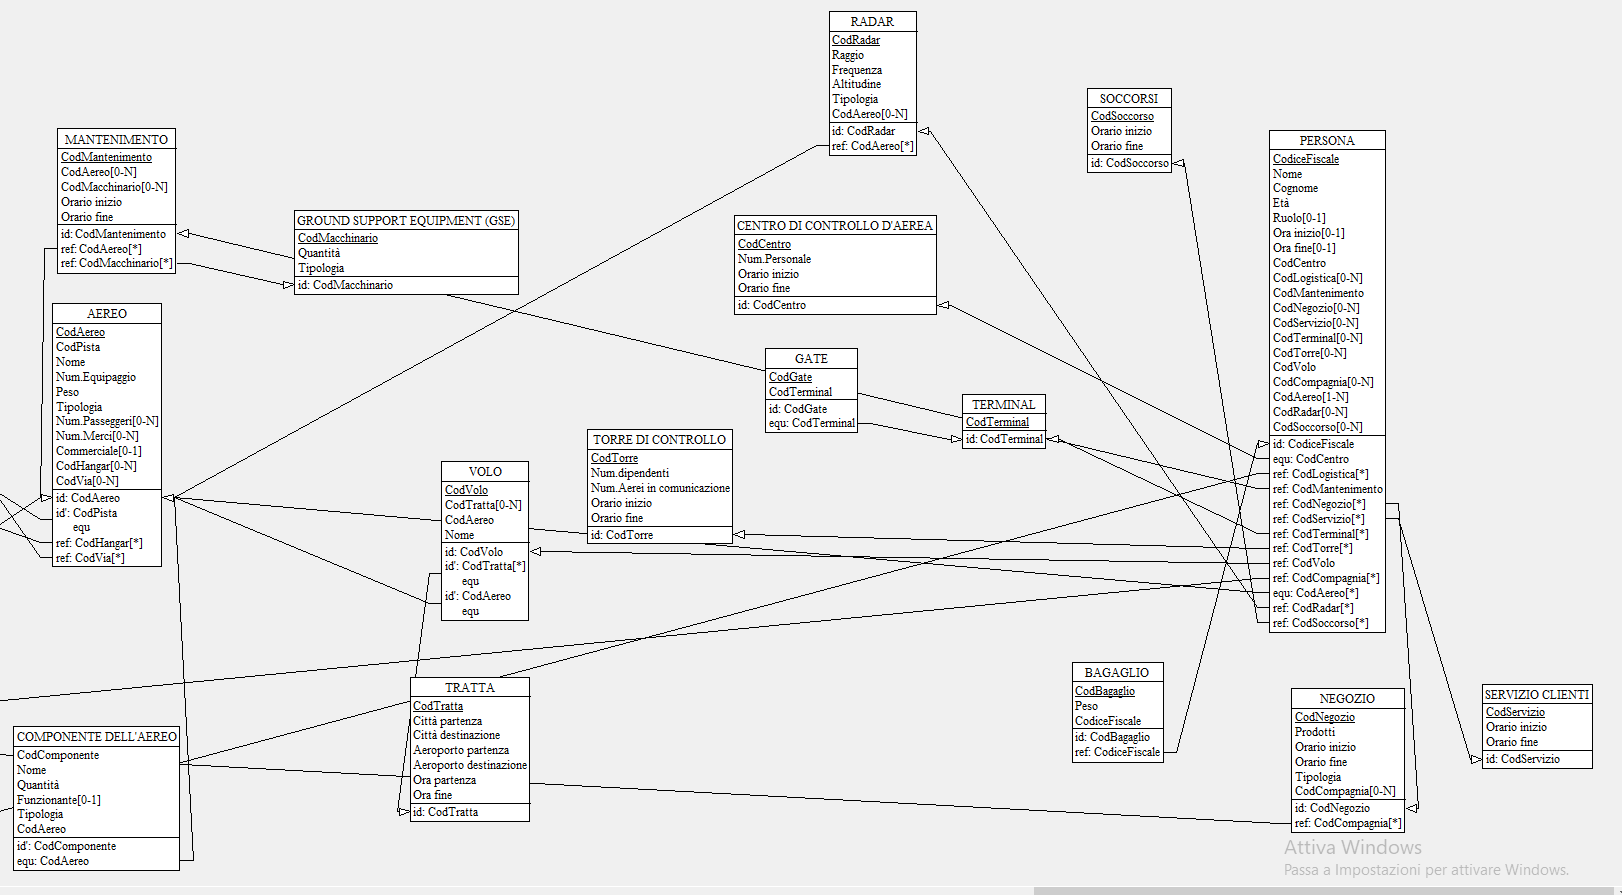
\includegraphics[width=1.2\textwidth]{./img/Schema_Logico/Schema_Logico1.png} %TODO: 1 o 1.1 o 1.2, con 1.2 perdiamo delle informazioni, ma si vedo meglio
	%\caption{}
	\label{fig:logico1}
\end{sidewaysfigure}
%\end{comment}

\begin{sidewaysfigure}[H]
	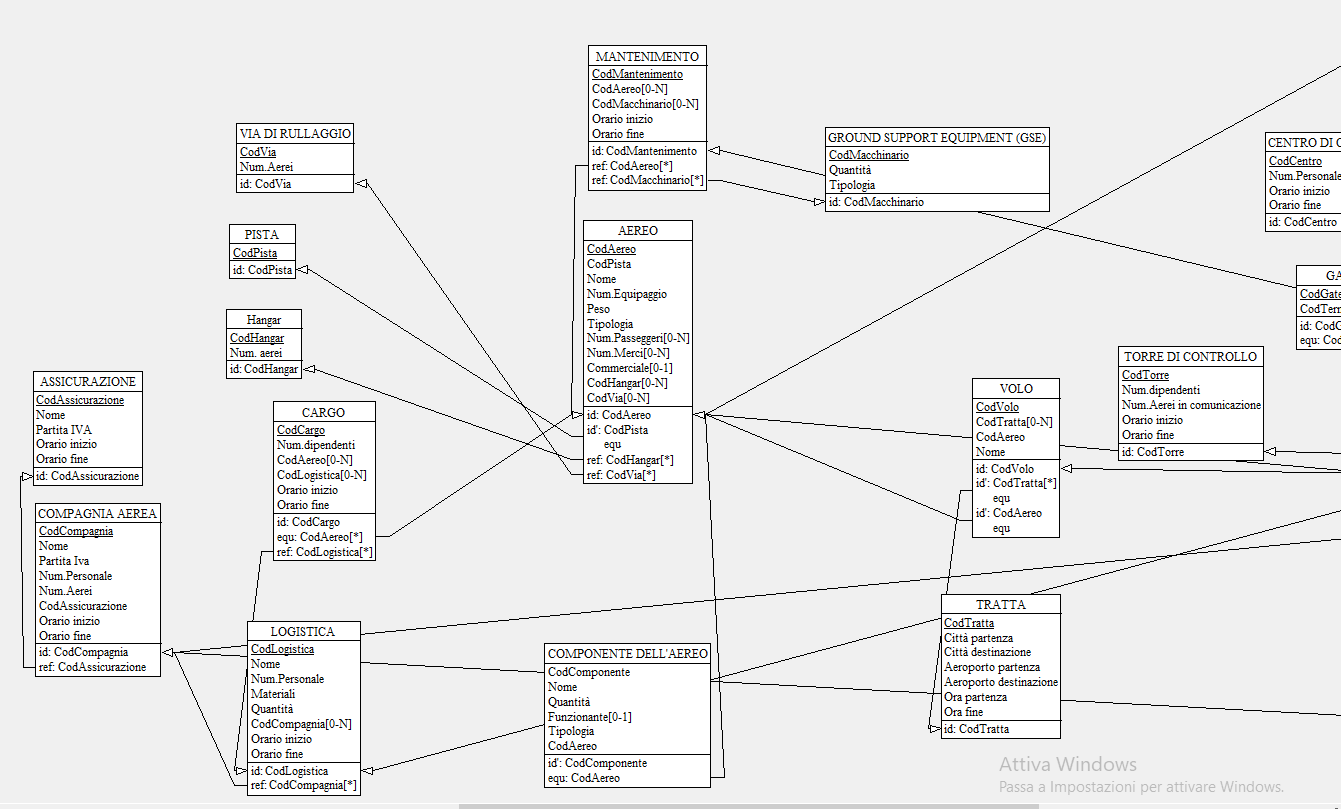
\includegraphics[width=1.2\textwidth]{./img/Schema_Logico/Schema_Logico2.png}
	%\caption{}
	\label{fig:logico2}
\end{sidewaysfigure}

\restoregeometry

% --------------- TRASFORMAZIONE DELLE OPERAZIONI IN QUERY SQL -----------------

\newpage

% oppure riproposizione delle operazioni in query sql
\subsection{Trasformazione delle operazioni in query SQL}

% OP 1 | Registrare un nuovo passeggero

\textbf{\small OP 1 | Registrare un nuovo passeggero}

%\begin{comment}
	
\begin{lstlisting}[language=SQL]
INSERT INTO aeroporto.persona (CodiceFiscale, CodBagaglio, Nome, Cognome, Età, CodVolo) VALUES(?, ?, ?, ?, ?, ?); 
\end{lstlisting} %TODO: fix Eta in Età

%\end{comment}
% OP 2 | Numero totale di componenti non funzionanti in un aereo.

\textbf{\small OP 2 | Numero totale di componenti non funzionanti in un aereo.}\\

\begin{lstlisting}[language=SQL]
SELECT COUNT(Funzionante) AS Num_Componenti_Non_Funzionanti
FROM aeroporto.aereo A JOIN aeroporto.componente_aereo CA ON A.CodAereo = CA.CodAereo
WHERE A.CodAereo = ?
AND CA.Funzionante = ?;
\end{lstlisting}

% OP 3 | Voli in partenza

\textbf{\small OP 3 | Voli in partenza}\\

\begin{lstlisting}[language=SQL]
SELECT volo.CodTratta, CodVolo, Nome, Città_partenza, Città_destinazione, Aeroporto_partenza, Aeroporto_destinazione, Ora_partenza, Ora_fine
FROM aeroporto.volo, aeroporto.tratta 
WHERE aeroporto.volo.CodTratta = aeroporto.tratta.CodTratta
AND aeroporto.tratta.Aeroporto_partenza = ?
AND Ora_Partenza = ?;
\end{lstlisting}

% OP 4 | Voli in arrivo

\textbf{\small OP 4 | Voli in arrivo}\\

\begin{lstlisting}[language=SQL]
SELECT volo.CodTratta, CodVolo, Nome, Città_partenza, Città_destinazione, Aeroporto_partenza, Aeroporto_destinazione, Ora_partenza, Ora_fine
FROM aeroporto.volo, aeroporto.tratta
WHERE aeroporto.volo.CodTratta = aeroporto.tratta.CodTratta
AND aeroporto.tratta.Aeroporto_destinazione = ?
AND Ora_fine = ?;	
\end{lstlisting}

% OP 5 | Manutenzione di un aereo

\textbf{\small OP 5 | Manutenzione di un aereo}\\

\begin{lstlisting}[language=SQL]
SELECT CodMantenimento, CodMacchinario, aeroporto.mantenimento.CodAereo
FROM aeroporto.mantenimento, aeroporto.aereo
WHERE aeroporto.mantenimento.CodAereo = aeroporto.aereo.CodAereo;	
\end{lstlisting}

% OP 6 | Comunicazioni tra controllori e membri dell'equipaggio di un aereo

\textbf{\small OP 6 | Comunicazioni tra controllori e membri dell'equipaggio di un aereo}\\

\begin{lstlisting}[language=SQL]
SELECT Num_Aerei_in_comunicazione
FROM aeroporto.torre_di_controllo
WHERE CodTorre = ?; 	
\end{lstlisting}

% OP 7 | Rifornimento di un aereo

%TODO: dalla 7 alla 14, scrivere qualche cosa.

\newpage %\pagebreak

\textbf{\small OP 7 | Rifornimento di un aereo}\\

\begin{lstlisting}[language=SQL]
SELECT *
FROM aeroporto.logistica, aeroporto.cargo
WHERE logistica.CodLogistica = cargo.CodLogistica
AND logistica.Materiali = ?;	
\end{lstlisting}

% OP 8 | Assunzione di nuovi addetti

\textbf{\small OP 8 | Assunzione di nuovi addetti}\\

\begin{lstlisting}[language=SQL]
INSERT INTO aeroporto.persona (CodiceFiscale, Nome, Cognome, Età, Ruolo, Ora_inizio, Ora_fine) VALUES (?, ?, ?, ?, ?, ?, ?);	
\end{lstlisting}

% OP 9 | 

\textbf{\small OP 9 | Operazioni di check-in }\\ %TODO: da finire

\begin{lstlisting}[language=SQL]
	
\end{lstlisting}

% OP 10 | 

\textbf{\small OP 10 | Aerei in pista}\\ %TODO: riguardarsela

\begin{lstlisting}[language=SQL]
SELECT Num_Aerei
FROM aeroporto.via_di_rullaggio
WHERE CodVia = ?;	
\end{lstlisting}

% OP 11 | Acquirenti ai negozi

\textbf{\small OP 11 | Acquirenti ai negozi}\\ %TODO: rimettere Persone che comprano prodotti ai negozi (o nei negozi).

\begin{lstlisting}[language=SQL]
SELECT COUNT(P.CodiceFiscale) AS Num_Clienti
FROM aeroporto.negozio N JOIN aeroporto.persona P on P.CodNegozio = N.CodNegozio
WHERE P.CodNegozio = ?;
\end{lstlisting}

% OP 12 | Passeggeri che si recano al Terminal
%TODO: meglio Persone o Passeggeri, teoricamente è più corretto Passeggeri.

\textbf{\small OP 12 | Persone che si recano al Terminal}\\

\begin{lstlisting}[language=SQL]
SELECT COUNT(P.CodiceFiscale) AS Persone_Al_Terminal
FROM aeroporto.terminal T JOIN aeroporto.persona P ON T.CodTerminal = P.CodTerminal
WHERE P.CodTerminal = ?;
\end{lstlisting}

% OP 13 | Nuovi membri dell'equipaggio assunti da una compagnia

\textbf{\small OP 13 | Nuovi membri dell'equipaggio assunti da una compagnia}\\

\begin{lstlisting}[language=SQL]
INSERT INTO aeroporto.persona ( CodiceFiscale, Nome, Cognome, Età, Ruolo, Ora_Inizio, Ora_fine, CodAereo )
VALUES ( ?, ?, ?, ?, ?, ?, ?, ? )	
\end{lstlisting}

% OP 14  | Inserimento di aerei stazionati negli Hangar

\textbf{\small OP 14 | Inserimento di aerei stazionati negli Hangar}\\

\begin{lstlisting}[language=SQL]
INSERT INTO aeroporto.aereo (CodAereo, CodPista, Nome, Num_Equipaggio, Peso, Tipologia, CodHangar) VALUES( ?, ?, ?, ?, ?, ?);	
\end{lstlisting}

% OP 15 | Calcolare l'età media dei passeggeri

\textbf{\small OP 15 | Calcolare l'età media dei passeggeri}\\

\begin{lstlisting}[language=SQL]
SELECT AVG(Età) AS Media_Età
FROM aeroporto.persona
WHERE Ruolo = "Passeggero";	
\end{lstlisting}

% OP 16  | Ottenere il numero di aerei di una compagnia aerea

\textbf{\small OP 16 | Ottenere il numero di aerei di una compagnia aerea}\\

\begin{lstlisting}[language=SQL]
SELECT Num_Aerei
FROM aeroporto.compagnia_aerea
WHERE CodCompagnia = ?;	
\end{lstlisting}

% OP 17  | Numero di controllori in una Torre di Controllo

\textbf{\small OP 17 | Numero di controllori in una Torre di Controllo}\\

\begin{lstlisting}[language=SQL]
SELECT Num_dipendenti
FROM aeroporto.torre_di_controllo
WHERE CodTorre = ?;	
\end{lstlisting}

% OP 18  | Numero di macchinari presenti nell'Aeroporto

\textbf{\small OP 18 | Numero di macchinari presenti nell'Aeroporto}\\

\begin{lstlisting}[language=SQL]
SELECT SUM(Quantità) AS Num_Totale_Macchinari
FROM aeroporto.ground_support_equipment;	
\end{lstlisting}

% OP 19  | Approvvigionamento dell'aereo

\textbf{\small OP 19 | Approvvigionamento dell'aereo}\\

\begin{lstlisting}[language=SQL]
SELECT CodiceFiscale, Nome, Cognome, Età, CodTorre, CodCentro, Ora_inizio, Ora_fine
FROM aeroporto.persona
WHERE Ruolo = "Controllore"
AND Ora_inizio >= CAST(? AS TIME)
AND Ora_fine <= CAST(? AS TIME)
GROUP BY Cognome;	
\end{lstlisting}

% OP 20  | Numero aerei commerciali di una compagnia aerea

\textbf{\small OP 20 | Numero aerei commerciali di una compagnia aerea}\\

\begin{lstlisting}[language=SQL]
SELECT COUNT(Commerciale) AS Num_Aerei_Commerciali
FROM aeroporto.aereo
WHERE Commerciale = ?;
\end{lstlisting}

% OP 21  | Quantità di merci trasportate in media da un aereo commerciale

\textbf{\small OP 21 | Quantità di merci trasportate in media da un aereo commerciale}\\

\begin{lstlisting}[language=SQL]
SELECT AVG(Num_Merci) AS Media_Merci_Trasportate
FROM aeroporto.aereo;	
\end{lstlisting}
	
	% ==================== PROGETTAZIONE DELL'APPLICATIVO ============================

\newpage

\enlargethispage{1\linewidth}

\section{Progettazione dell'Applicativo}

\textsf{\small L'applicativo per poter interagire con la base di dati è stato sviluppato in \textbf{JavaFX}, usufruendo dello strumento di creazione di interfaccie grafiche \textbf{Scene Builder}. }\\

\textsf{\small Per quanto riguarda l'immagazzinamento del database è stato eseguito in locale con \textbf{MySQL}.}\\

\begin{figure}[ht] 
	\centering
	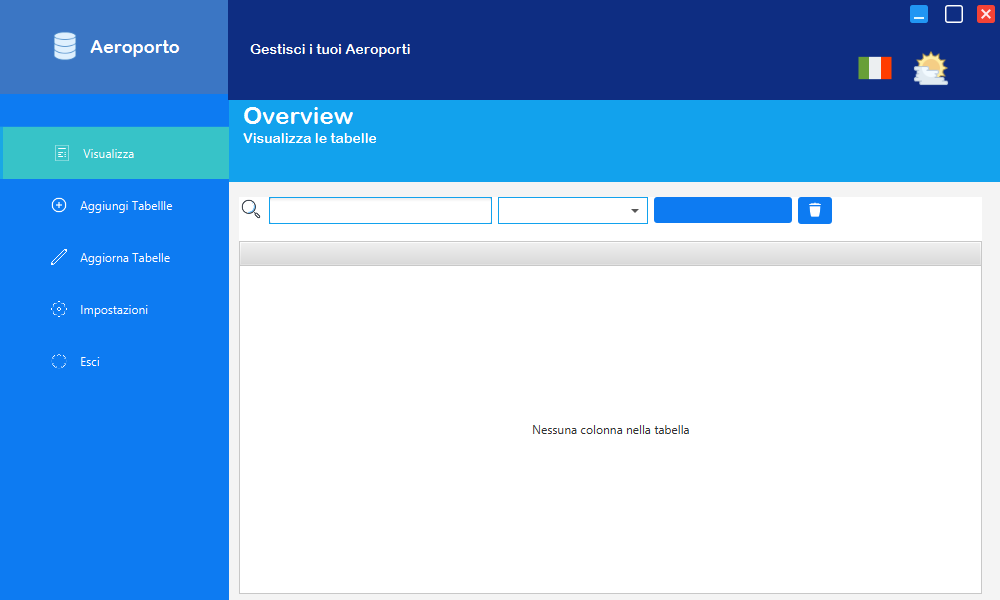
\includegraphics[width=1\textwidth, height=1\textheight, keepaspectratio]{./img/Applicativo/homepage.png}
	\caption{Homepage dell'Applicativo.}
	\label{fig:homepage}
\end{figure}

\textsf{\small Esso presenta svariate funzionalità necessarie per l'interazione col database e opzionali: } 

\begin{itemize}
	\item \textsf{\small Visualizzazione delle tabelle.}
	\item \textsf{\small Aggiunta di righe nelle tabelle.}
	\item \textsf{\small Modifica dei dati delle righe.}
	\item \textsf{\small Rimozione di specifiche righe selezionate dall'utente.}
	\item \textsf{\small Messaggi per notificare l'utente sull'esecuzione o meno dell'operazione scelta.}
	\item \textsf{\small Barra di ricerca per poter trovare gli elementi di una tabella più facilmente.}
	\item \textsf{\small Possibilità di modificare la lingua in Inglese o in Italiano.}
	\item \textsf{\small Possibilità di modificare il tema del software in chiaro o scuro.}
	\item \textsf{\small Possibilità di salvare la lingua e il tema scelti in un file di impostazioni sicuro criptato tramite lo \emph{Advanced Encryption Standard} (\textbf{AES}).}
	\item \textsf{\small Possibilità di resettare le impostazioni di default.}
	%\item \textsf{\small }
\end{itemize}

% ========================== OVERVIEW ==========================================

\newpage

\enlargethispage{1\linewidth}

\subsection{Overview | Visualizza}

\textsf{\small Questa schermata permette all'utente in base ad una scelta dal \emph{combo box} di poter selezionare la tabella da visionare. (L'immagine \ref{fig:maximize} fa uso del tema scuro e della lingua inglese)}\\

\begin{figure}[ht]
	\begin{subfigure}{.6\textwidth}
		\centering
		%\flushleft
		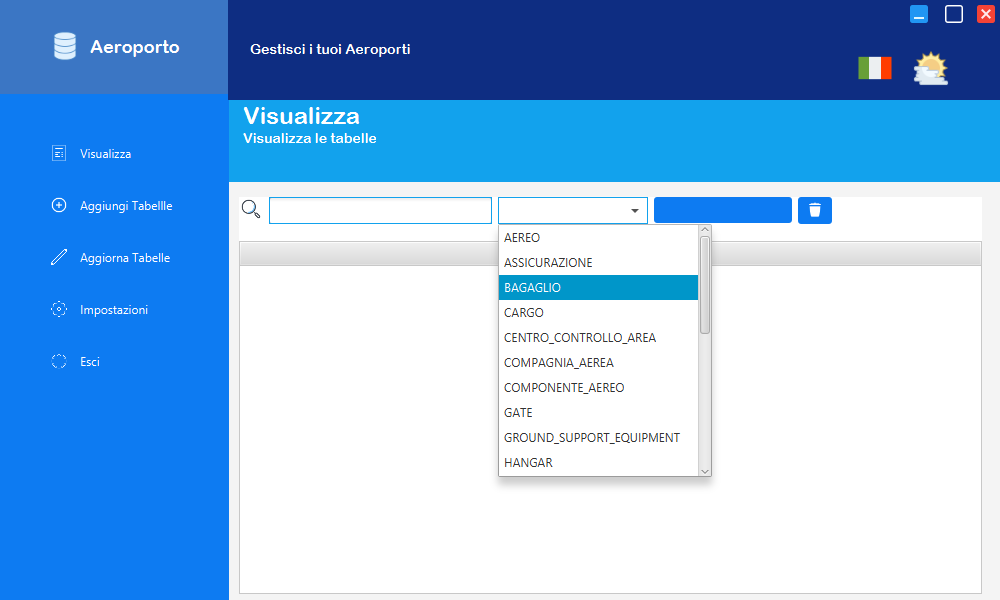
\includegraphics[width=1\linewidth]{./img/Applicativo/homepage_overview_table_selection.png}
		\caption{Selezione tabella}
		\label{fig:overview1}
	\end{subfigure}%
	\begin{subfigure}{.6\textwidth}
		\centering
		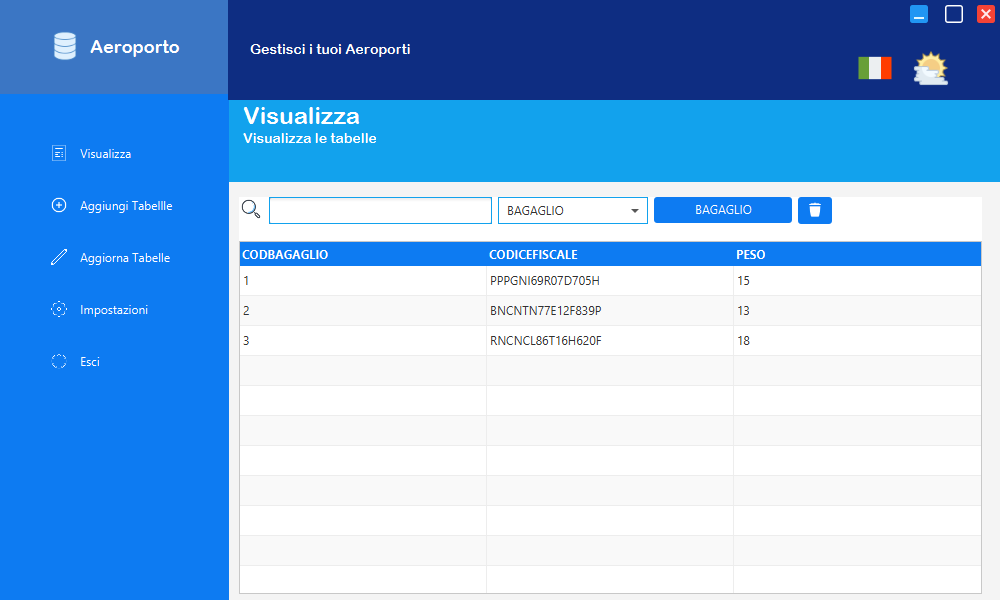
\includegraphics[width=1\linewidth]{./img/Applicativo/homepage_overview_table_selection2.png}
		\caption{Visualizzazione tabella selezionata}
		\label{fig:overview2}
	\end{subfigure}
	%\caption{a}
	\label{fig:overviews}
\end{figure}


\begin{figure}[H] 
\centering
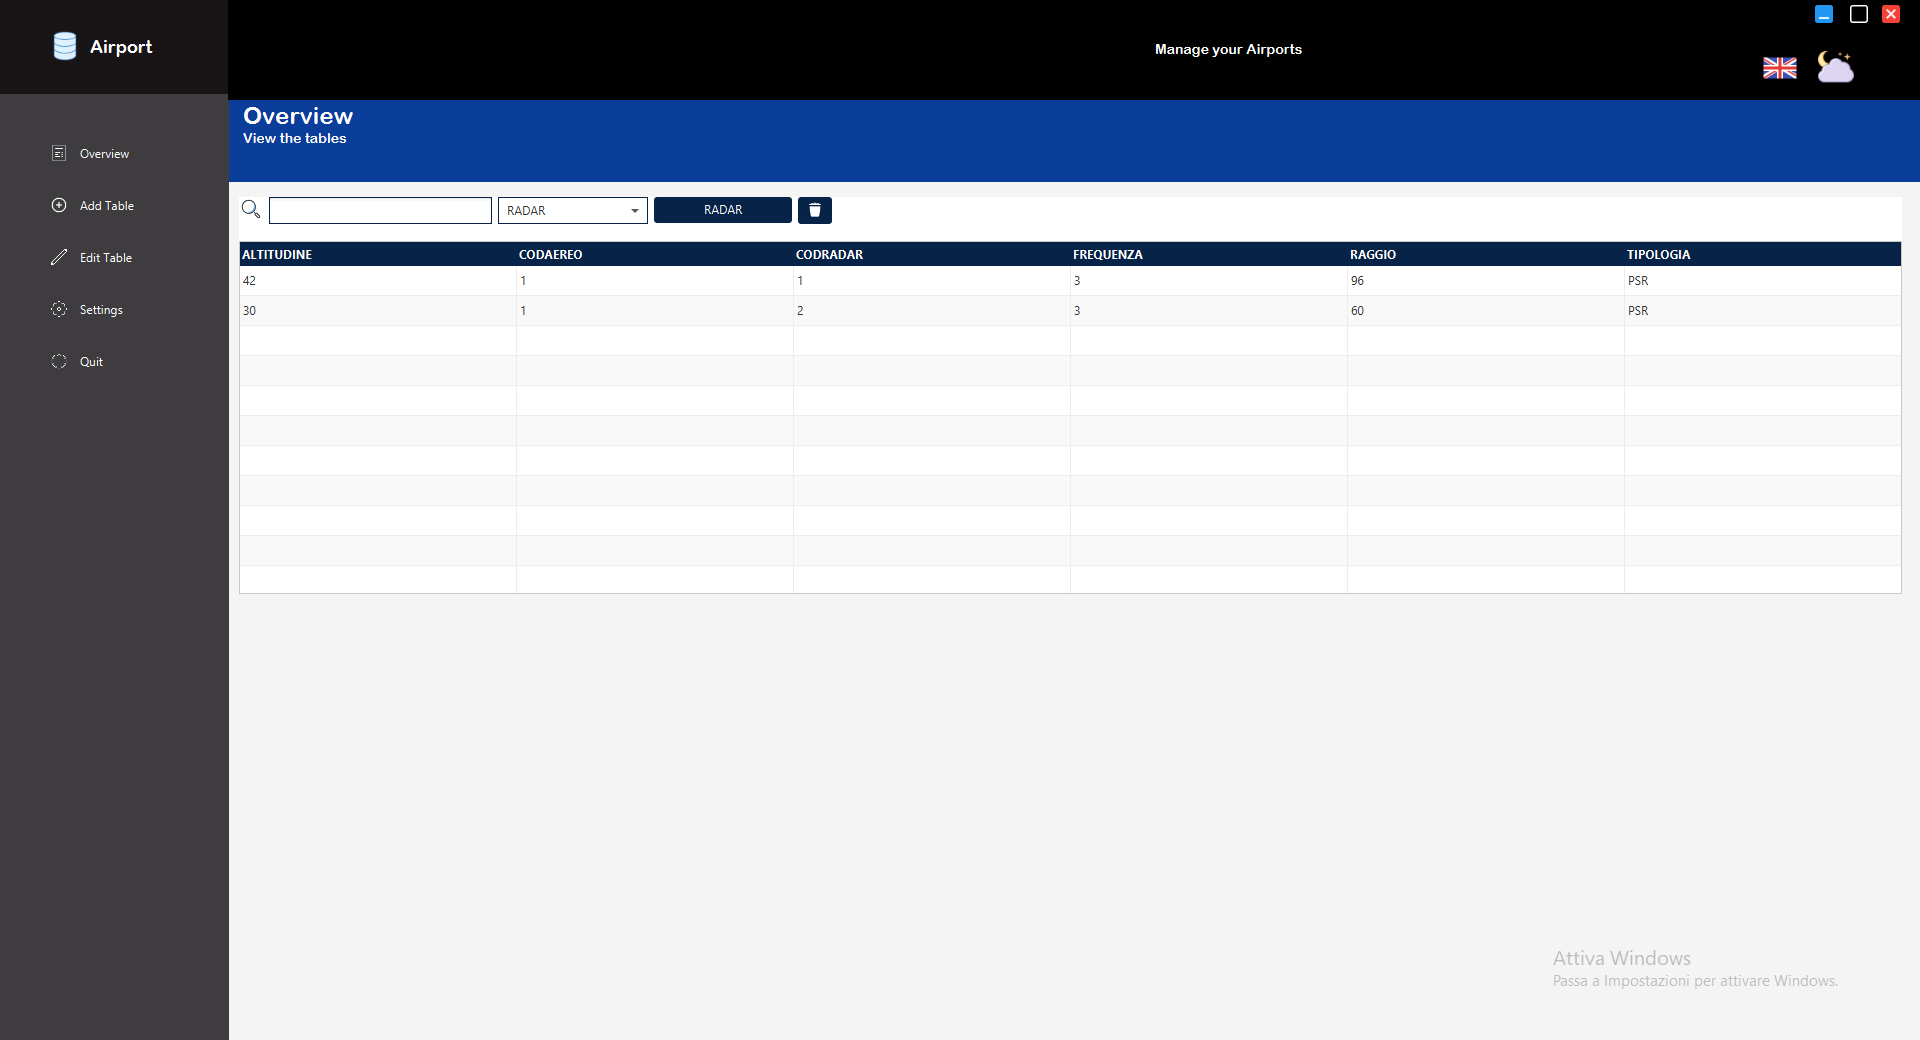
\includegraphics[width=1\textwidth, height=1\textheight, keepaspectratio]{./img/Applicativo/maximize.png}
\caption{Homepage dell'Applicativo schermata massimizzata.}
\label{fig:maximize}
\end{figure}


\textsf{\small Inoltre son presenti due ulteriori funzionalità: quella di poter ricercare elementi dalla barra di ricerca e quella di poter eliminare una determinata riga selezionata di una tabella.}\\

% ========================== SEARCH BAR =======================================

\pagebreak

%\enlargethispage{1\linewidth}

\subsubsection{Search Bar | Barra di Ricerca}

\textsf{\small La barra di ricerca trova tutti gli elementi scritti in essa. Se una data informazione si trova in più righe allora mostra tutte le righe, altrimenti solo una oppure nessuna se il dato cercato non è presente nella tabella in questione.}

\begin{figure}[H] 
	\centering
	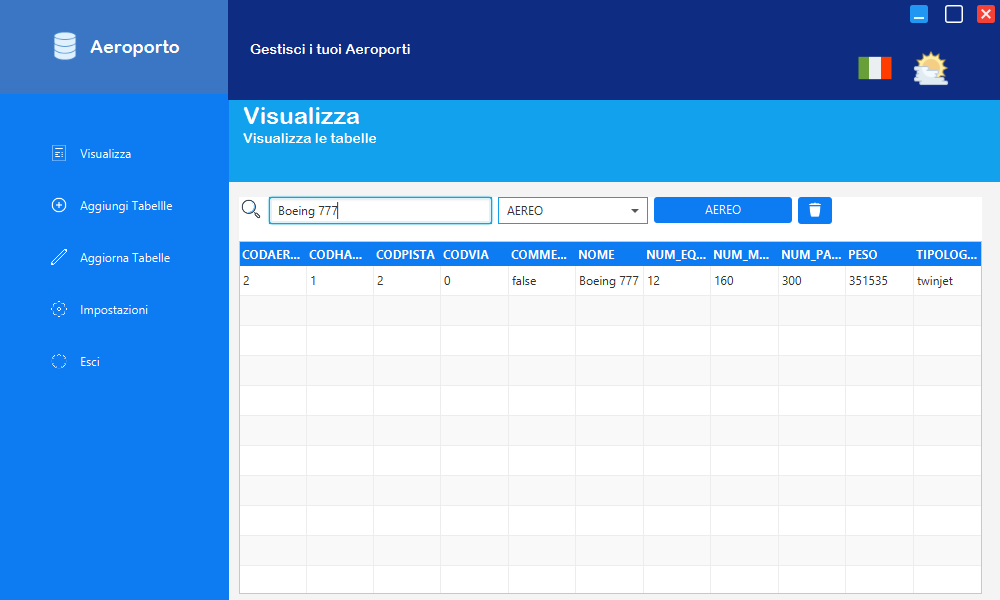
\includegraphics[width=1\textwidth, height=1\textheight, keepaspectratio]{./img/Applicativo/search_bar2.png}
	\caption{Ricerca di uno specifico aereo.}
	\label{fig:search_bar2}
\end{figure}

\begin{figure}[H]
	\begin{subfigure}{.6\textwidth}
		\centering
		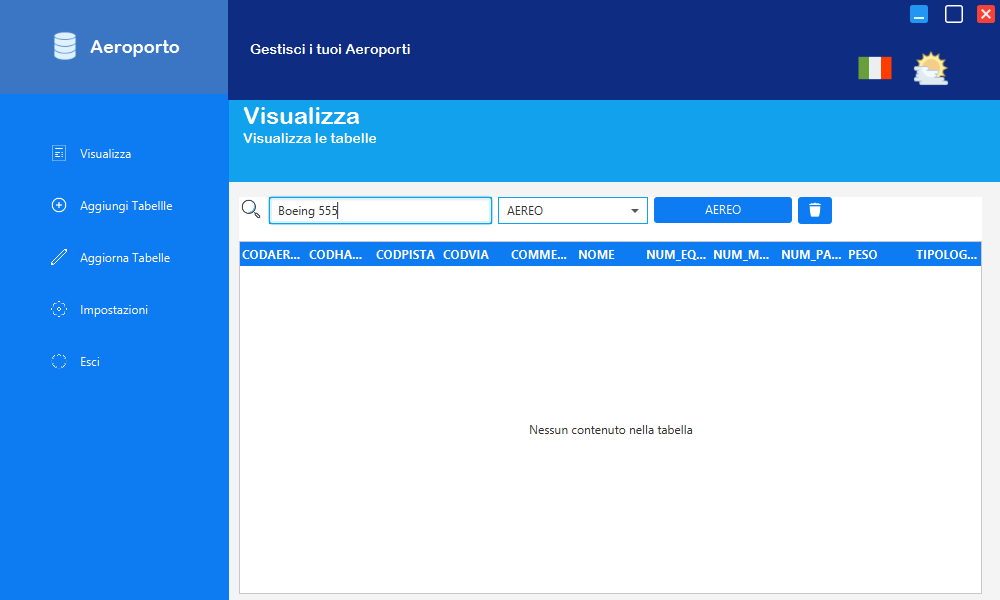
\includegraphics[width=1\linewidth]{./img/Applicativo/search_bar3.png}
		\caption{Ricerca non trovata perchè elemento non presente.}
		\label{fig:search_bar3}
	\end{subfigure}%
	\begin{subfigure}{.6\textwidth}
		\centering
		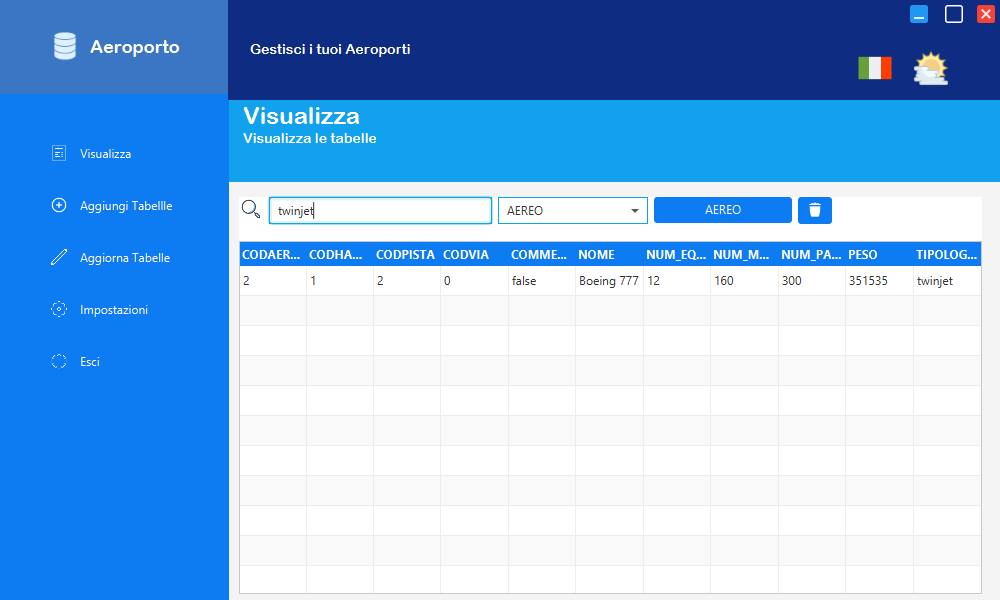
\includegraphics[width=1\linewidth]{./img/Applicativo/search_bar4.png}
		\caption{Ricerca trovata}
		\label{fig:search_bar4}
	\end{subfigure}
	%\caption{a}
	\label{fig:search_bars}
\end{figure}

\begin{figure}[H]
	\begin{subfigure}{.6\textwidth}
		\centering
		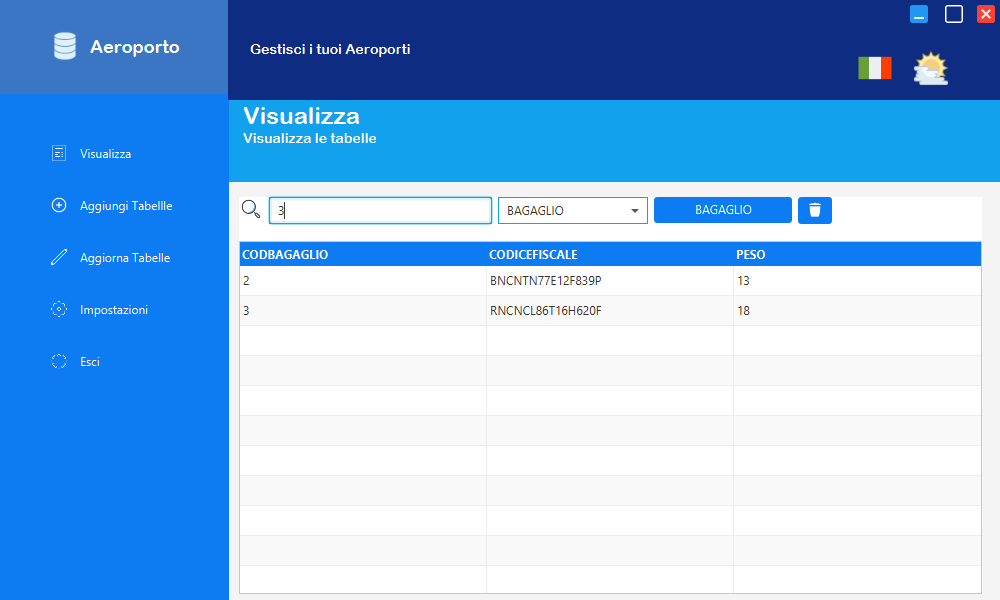
\includegraphics[width=1\linewidth]{./img/Applicativo/search_bar7.png}
		\caption{Trovati due elementi con quelle specifiche}
		\label{fig:search_bar7}
	\end{subfigure}%
	\begin{subfigure}{.6\textwidth}
		\centering
		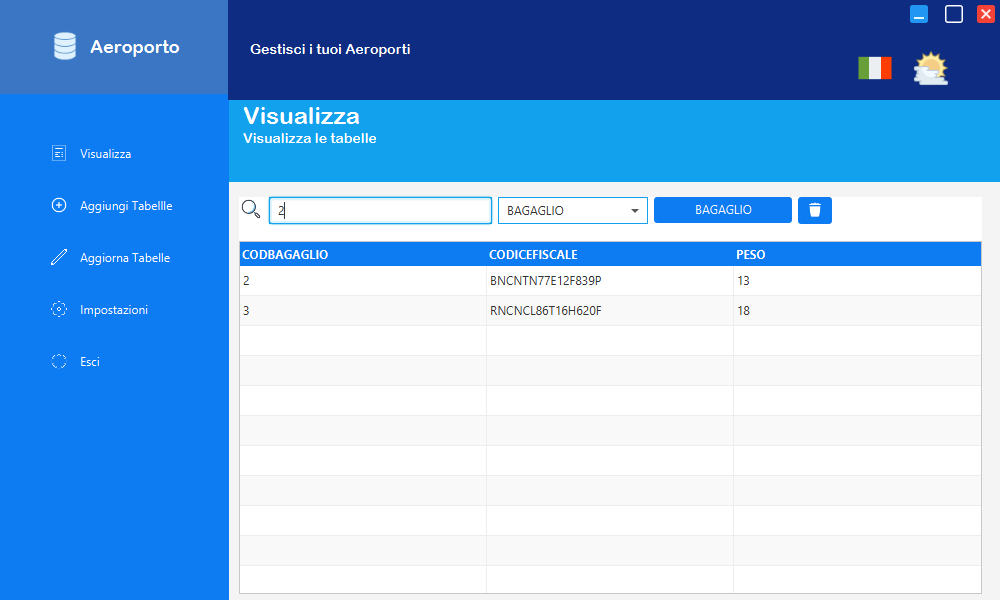
\includegraphics[width=1\linewidth]{./img/Applicativo/search_bar8.png}
		\caption{Trovati due elementi con quelle specifiche}
		\label{fig:search_bar8}
	\end{subfigure}
	%\caption{a}
	\label{fig:search_bars2}
\end{figure}

% ========================== DELETE ===========================================

%\pagebreak

\enlargethispage{1\linewidth}

\subsubsection{Delete | Rimozione}

\textsf{\small Tramite l'interruttore \emph{Cancella}, quello con l'icona del cestino, una volta selezionata la riga e aver confermato l' \emph{Alert} che chiede all'utente se è sicuro di voler procedere, l'elemento verrà cancellato.}

\begin{figure}[H] 
	\centering
	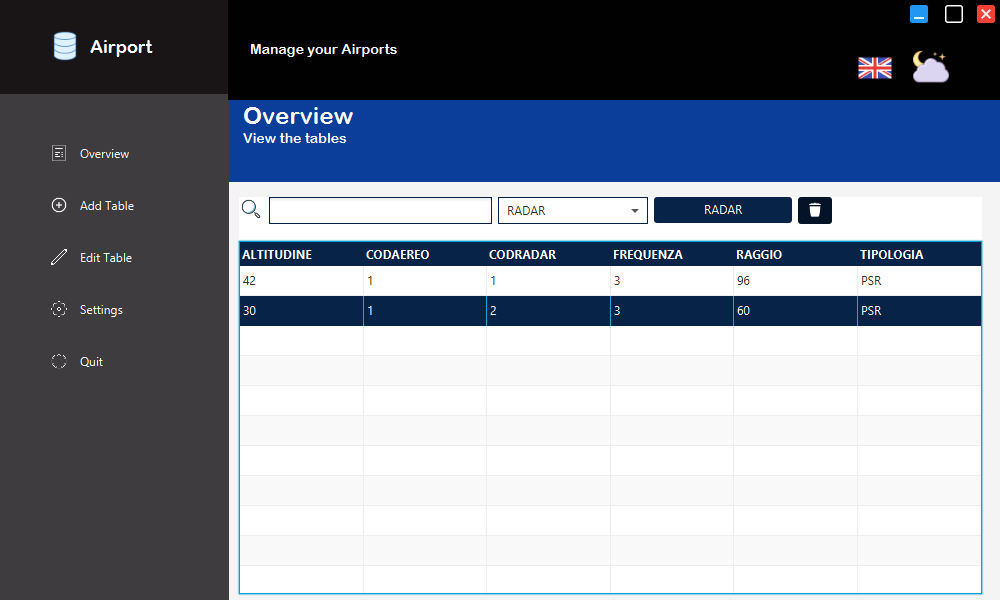
\includegraphics[width=1\textwidth, height=1\textheight, keepaspectratio]{./img/Applicativo/delete_data.png}
	\caption{Cancellazione della suddetta riga di dati.}
	\label{fig:delete_data}
\end{figure}

\pagebreak

\begin{figure}[H] 
	\centering
	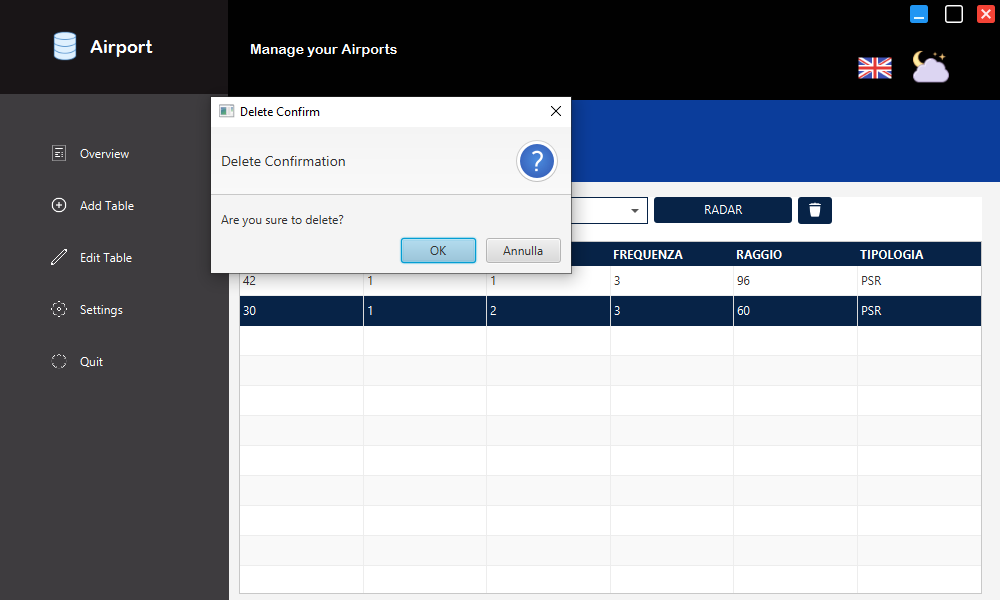
\includegraphics[width=1\textwidth, height=1\textheight, keepaspectratio]{./img/Applicativo/delete_alert_confirmation.png}
	\caption{Conferma cancellazione Alert.}
	\label{fig:delete_alert_confirmation}
\end{figure}

%\pagebreak

\begin{figure}[H]
	\begin{subfigure}{.6\textwidth}
		\centering
		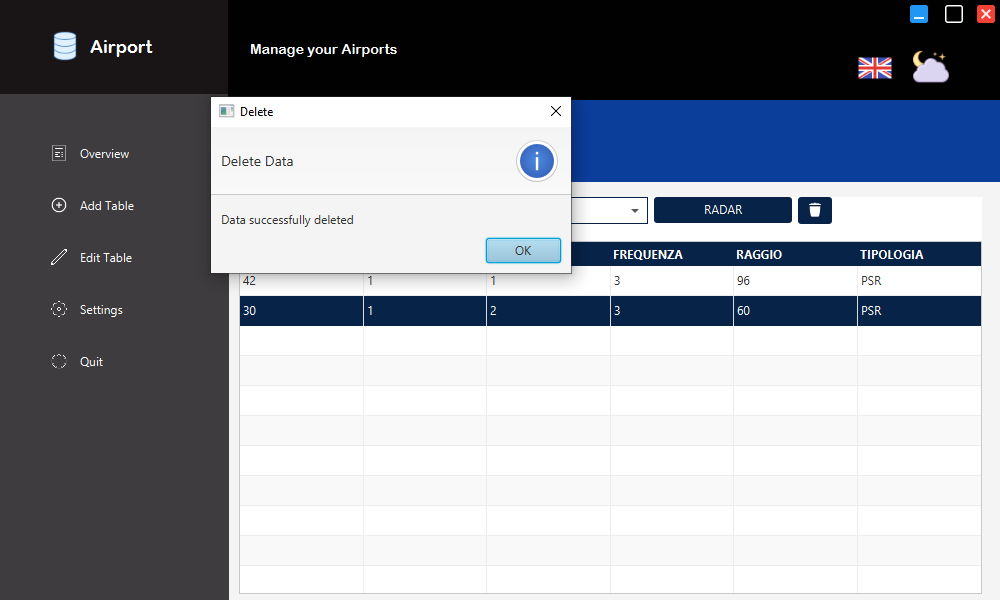
\includegraphics[width=1\linewidth]{./img/Applicativo/delete_data_success.png}
		\caption{Alert eliminazione con successo}
		\label{fig:delete_alert_success}
	\end{subfigure}%
	\begin{subfigure}{.6\textwidth}
		\centering
		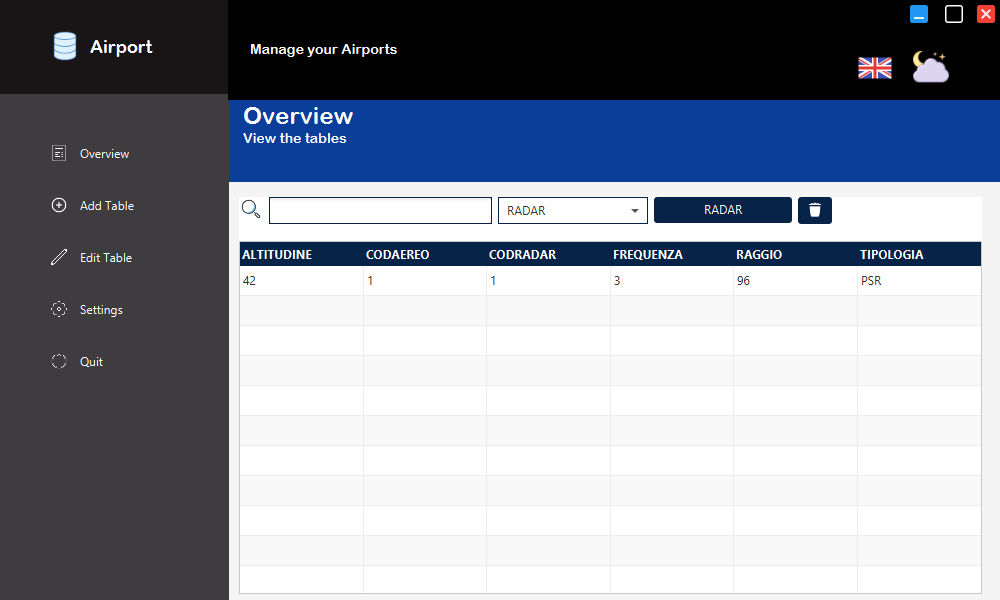
\includegraphics[width=1\linewidth]{./img/Applicativo/delete_data_aftermath.png}
		\caption{Visualizzazione della tabella dopo la cancellazione}
		\label{fig:delete_data_aftermath}
	\end{subfigure}
	%\caption{a}
	\label{fig:overviews2}
\end{figure}

% ========================== ADD TAB ==========================================

\newpage

\subsection{Add | Aggiungi}

\textsf{\small La scheda Aggiungi permette all'utente, una volta selezionata una tabella, attraverso i campi di testo di aggiungere una riga di dati alla tabella in questione.}\\

\begin{figure}[H] 
	\centering
	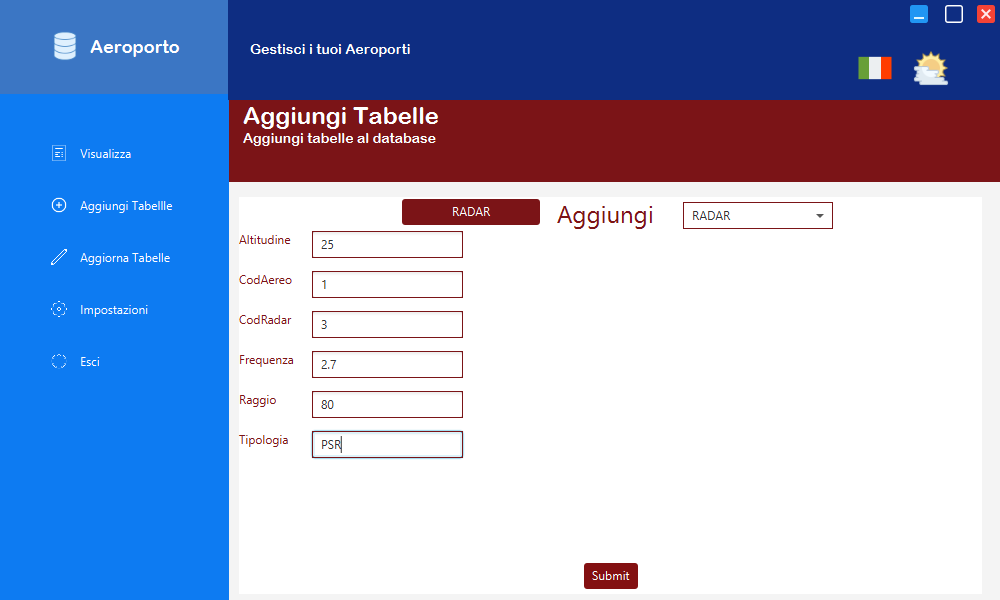
\includegraphics[width=1\textwidth, height=1\textheight, keepaspectratio]{./img/Applicativo/add_table.png}
	\caption{Aggiunta riga con i text fields.}
	\label{fig:add_table}
\end{figure}

\textsf{\small Dopo che l'utente avrà riempito i boxes e avrà premuto il pulsante \emph{Submit} l'operazione verrà eseguita e un \emph{Alert} lo notificherà se è andata a successo o se si sono verificati degli errori. (Nell'immagine \ref{fig:add_alert_error} viene mostrata la schermata con l'utilizzo del tema scuro) }\\

\begin{figure}[ht]
	\begin{subfigure}{.6\textwidth}
		\centering
		%\flushleft
		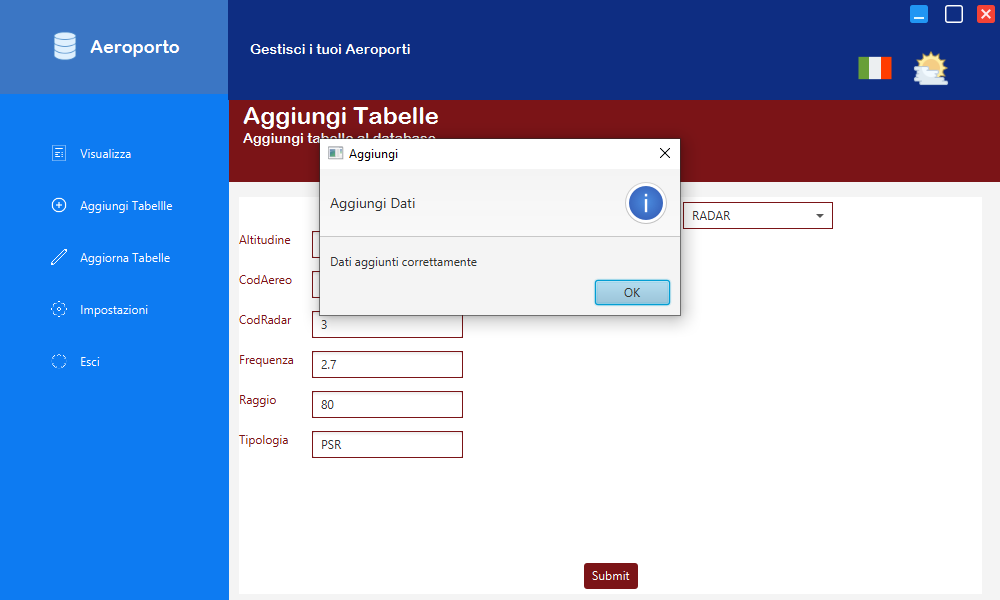
\includegraphics[width=1\linewidth]{./img/Applicativo/add_table_alert_success.png}
		\caption{Alert operazione eseguita con successo}
		\label{fig:add_alert_success}
	\end{subfigure}%
	\begin{subfigure}{.6\textwidth}
		\centering
		%\flushleft
		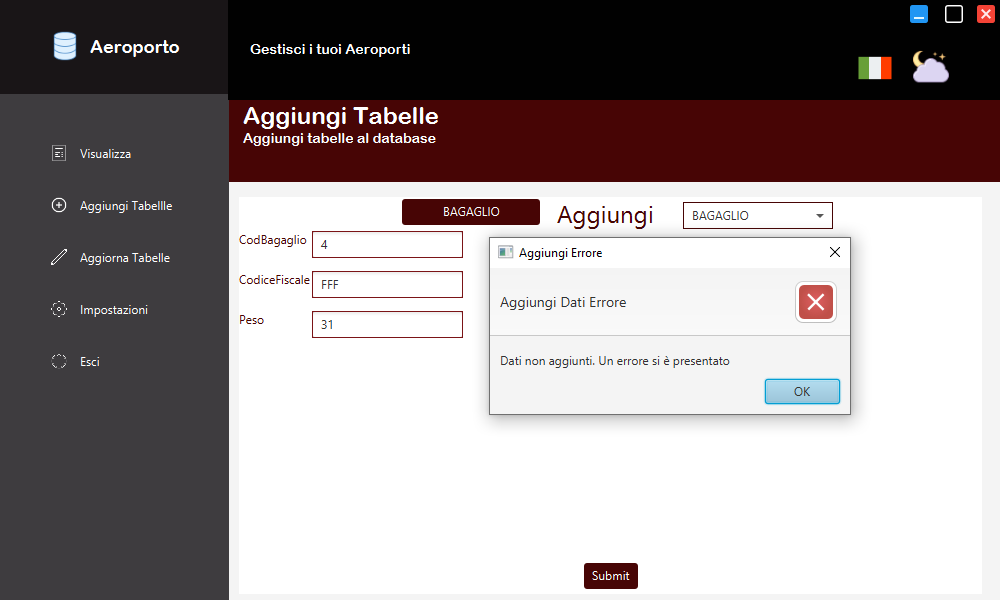
\includegraphics[width=1\linewidth]{./img/Applicativo/add_table_alert_error.png}
		\caption{Alert operazione non eseguita. Errori presenti}
		\label{fig:add_alert_error}
	\end{subfigure}
	%\caption{Add Tab Alerts}
	\label{fig:adds}
\end{figure}

% ========================== EDIT TAB ==========================================

\newpage

\enlargethispage{1\linewidth}

\subsection{Edit | Modifica}

\textsf{\small Tramite questa schermata, una volta scelta la tabella da modificare, dei campi di testo compariranno sulla sinistra.}\\

\begin{figure}[H] 
	\centering
	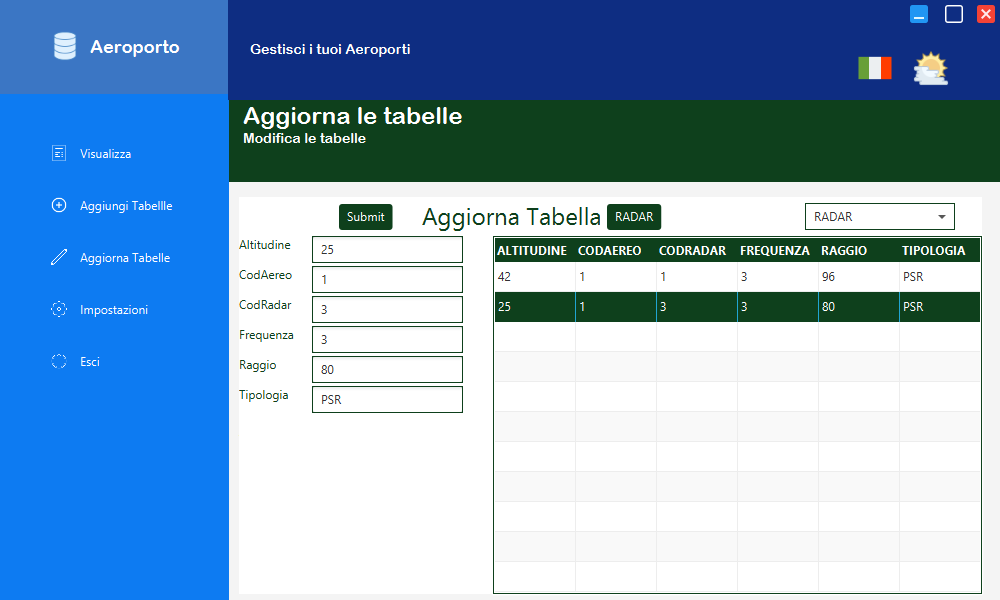
\includegraphics[width=1\textwidth, height=1\textheight, keepaspectratio]{./img/Applicativo/edit_table.png}
	\caption{Selezionata riga e dati automaticamente presentati nei text fields.}
	\label{fig:edit_table1}
\end{figure}

\textsf{\small Una volta selezionata la riga della tabella che si vuole editare i dati compariranno nei campi di testo e potranno essere modificati dall'utente.}\\

\begin{figure}[H] 
	\centering
	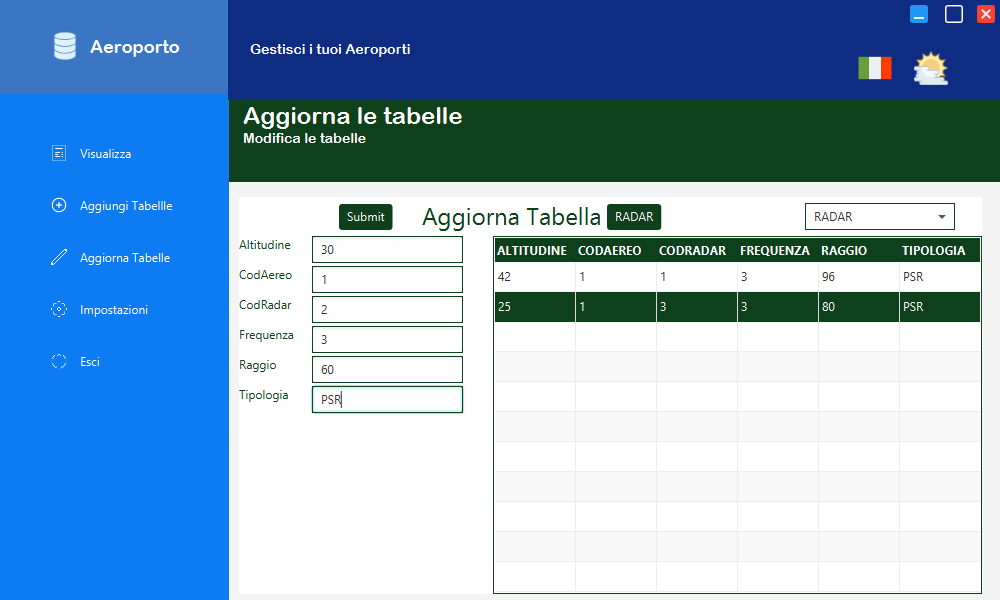
\includegraphics[width=1\textwidth, height=1\textheight, keepaspectratio]{./img/Applicativo/edit_table2.png}
	\caption{Modifica dei dati attraverso i text fields.}
	\label{fig:edit_table2}
\end{figure}

\pagebreak

\enlargethispage{1\linewidth}

\textsf{\small Come per la precedente operazione, una volta premuto \emph{Submit} un \emph{Alert} comparirà e avviserà l'utente. (Nell'immagine \ref{fig:edit_table_alert_error} è stata modificata la lingua in inglese e l'alert viene mostrato in quella lingua)}\\

\begin{figure}[H] 
	\centering
	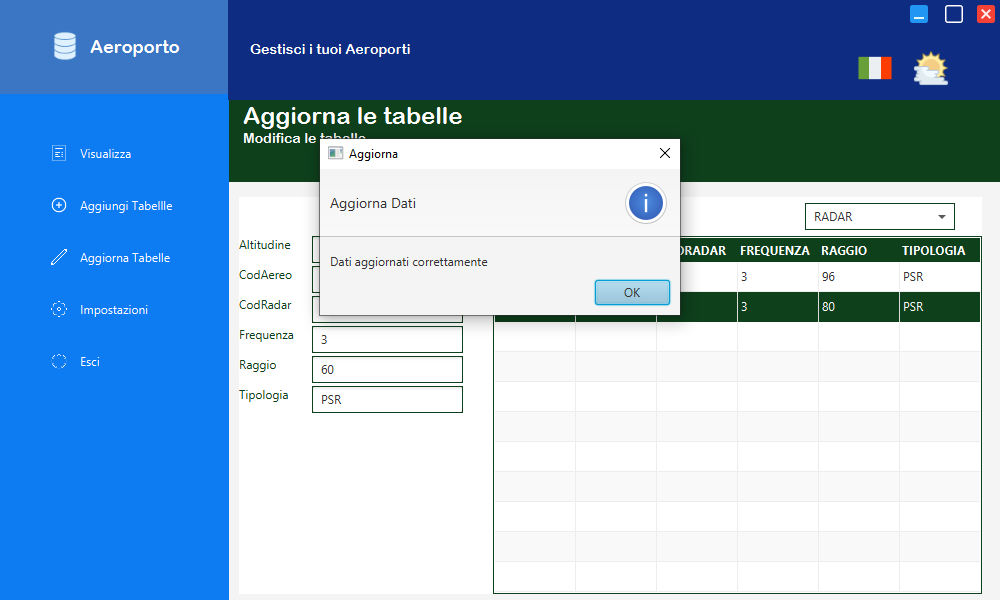
\includegraphics[width=1\textwidth, height=1\textheight, keepaspectratio]{./img/Applicativo/edit_table_alert.png}
	\caption{Alert operazione modifica eseguita con successo.}
	\label{fig:edit_table_alert_success}
\end{figure}

\begin{figure}[H] 
	\centering
	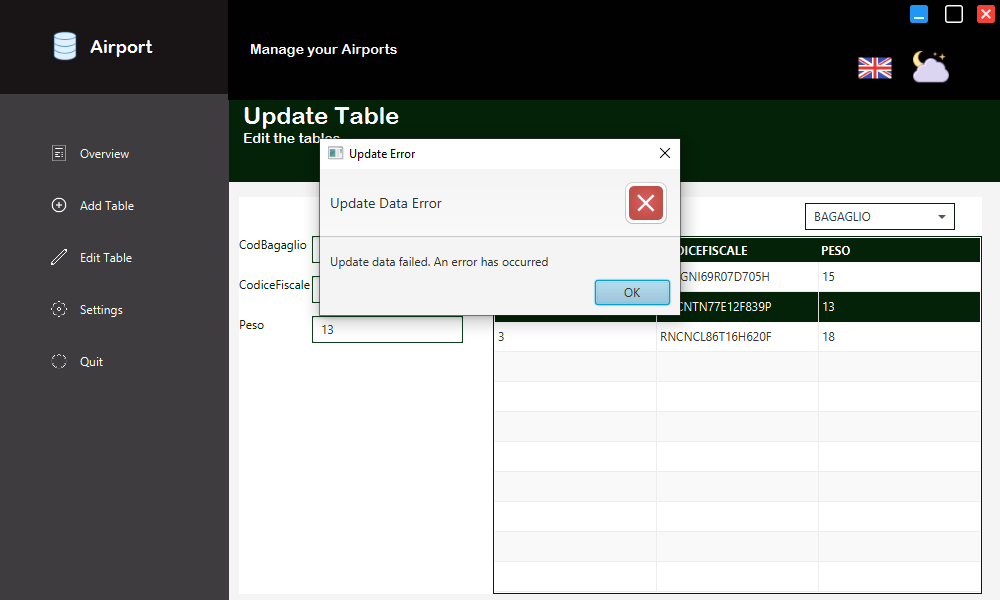
\includegraphics[width=1\textwidth, height=1\textheight, keepaspectratio]{./img/Applicativo/edit_table_alert_error.png}
	\caption{Alert operazione modifica eseguita con successo.}
	\label{fig:edit_table_alert_error}
\end{figure}

% ========================== SETTINGS TAB =====================================

\newpage

\enlargethispage{1\linewidth}

\subsection{Settings | Impostazioni}

\textsf{\small Questa è la pagina delle impostazioni, ce ne sono due possibili, questa sono la Lingua e il Tema del software.}

\begin{figure}[H] 
	\centering
	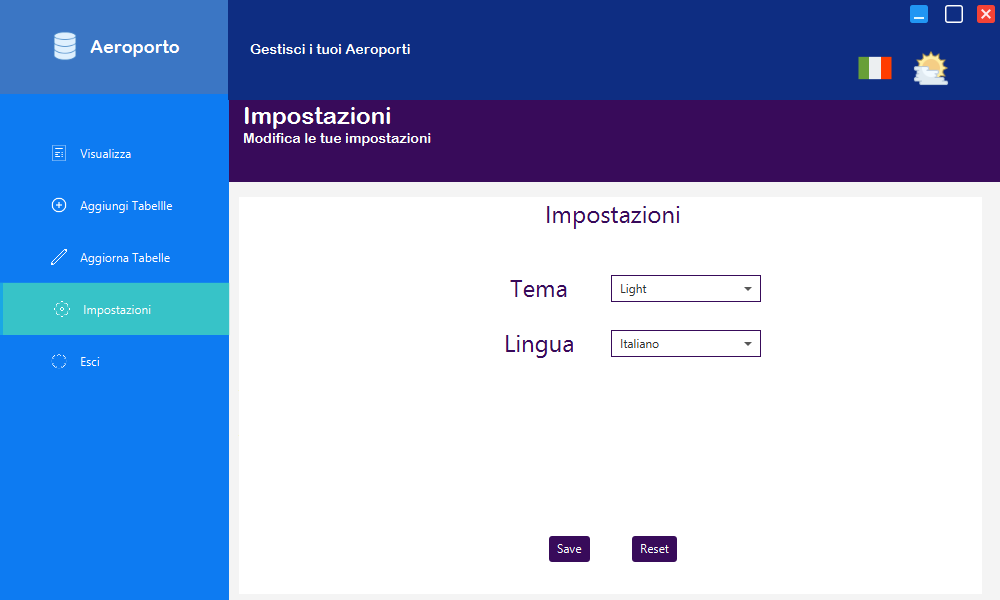
\includegraphics[width=1\textwidth, height=1\textheight, keepaspectratio]{./img/Applicativo/settings.png}
	\caption{Pannello delle Impostazioni.}
	\label{fig:settings1}
\end{figure}

\textsf{\small Queste possono essere modificate qui, nel pannello delle impostazioni oppure semplicemente cliccando le rispettive icone in alto a destra, in questo modo l'impostazione attuale verrà cambiata con l'altra possibile impostazione.}

\begin{figure}[H] 
	\centering
	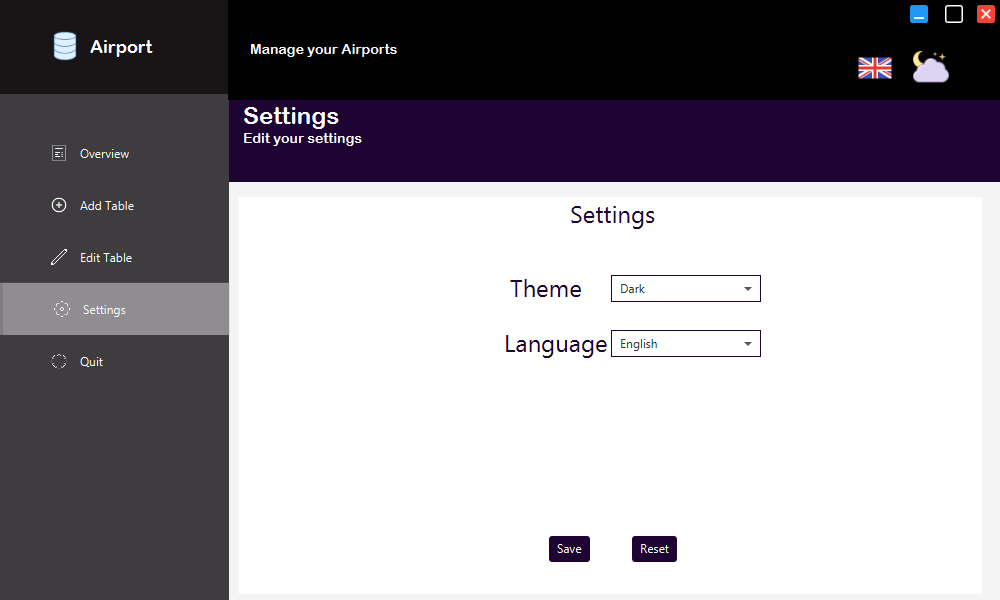
\includegraphics[width=1\textwidth, height=1\textheight, keepaspectratio]{./img/Applicativo/settings_change_language_and_theme.png}
	\caption{Impostazioni modificate e in tempo reale i cambiamenti vengono attuati.}
	\label{fig:settings2}
\end{figure}

% ========================== SAVE TAB =========================================

\pagebreak

\enlargethispage{1\linewidth}

\subsubsection{Save | Salvataggio}

\textsf{\small Attraverso il tasto \emph{Save} potranno essere salvate le impostazioni selezionate nei due combo box.}\\

\begin{figure}[H] 
	\centering
	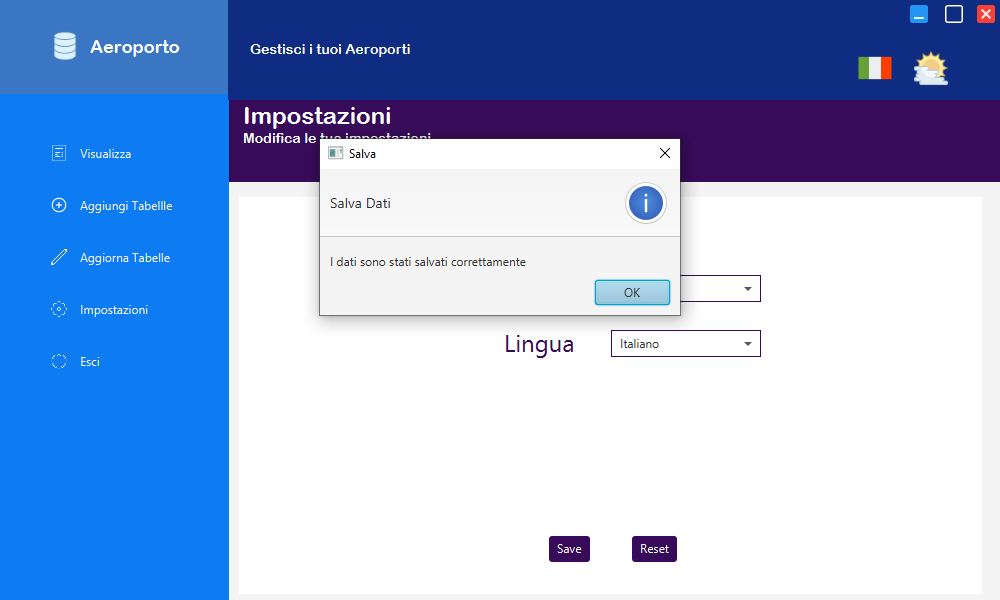
\includegraphics[width=1\textwidth, height=1\textheight, keepaspectratio]{./img/Applicativo/salvataggio.png}
	\caption{Salvataggio delle impostazioni e alert di conferma}
	\label{fig:save_alert_success}
\end{figure}

\textsf{\small Col pulsante \emph{Reset} si potrà resettare le impostazioni a quelle di default, ovvero Lingua : \emph{Inglese} e Tema : \emph{Chiaro}. Questo pulsante però, si limita a cambiare le impostazioni nei combo box e nelle icone, ma non a salvarle.}\\

\textsf{\small Queste impostazioni vengono salvate in un file JSON chiamato \emph{settings.dat} e criptato attraverso l' \emph{Advanced Encryption Standard} (\textbf{AES}).}\\

\begin{figure}[H] 
	\centering
	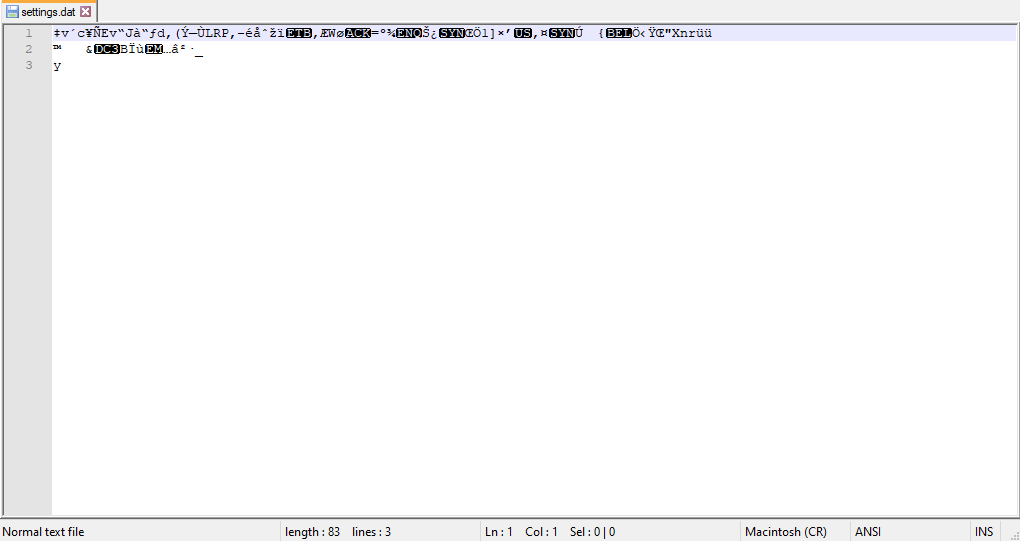
\includegraphics[width=1\textwidth, height=1\textheight, keepaspectratio]{./img/Applicativo/salvataggio_criptato.png}
	\caption{Salvataggio delle impostazioni e alert di conferma}
	\label{fig:encrypted_save_file}
\end{figure}

% ========================== QUIT TAB =========================================

\newpage

\subsection{Quit | Uscita}

\textsf{\small Infine, l'ultima sezione del software è l'uscita dal programma possibile sia dall'icone della crocetta rossa in alto a destra (che però non utilizza un Alert) sia dal menù \emph{Quit | Uscita} e dopo aver confermato l'uscita dall' \emph{Alert} si uscirà dal programma.}\\

\begin{figure}[H] 
	\centering
	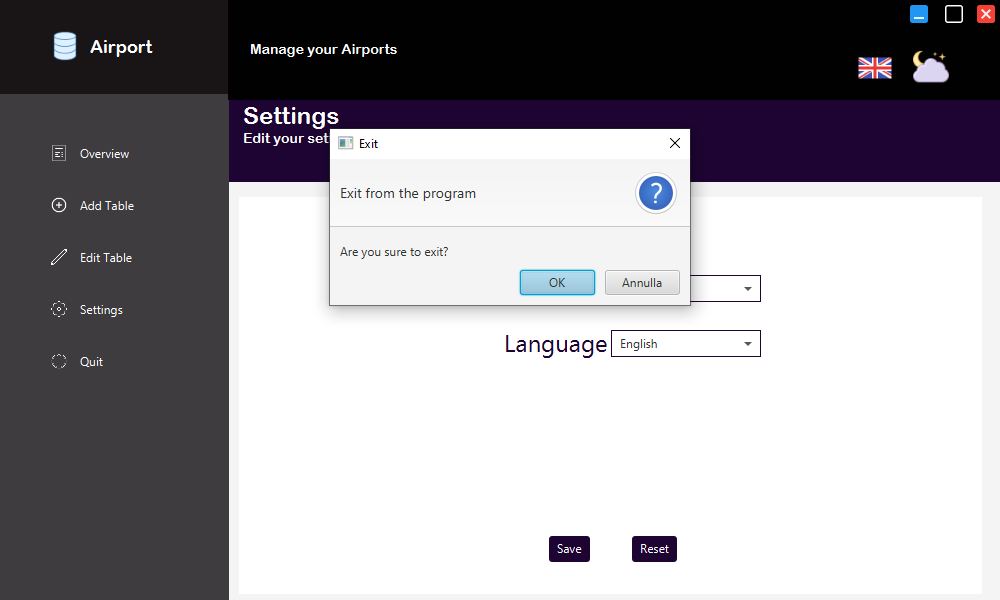
\includegraphics[width=1\textwidth, height=1\textheight, keepaspectratio]{./img/Applicativo/quit_alert.png}
	\caption{Alert di conferma per l'uscita}
	\label{fig:quit_alert}
\end{figure}
	
	% ==================== GUIDA ALL'UTILIZZO ==========================================

\newpage

\enlargethispage{1\linewidth}

\section{Guida all'Utilizzo}

\textsf{\small Qui, di seguito verranno indicate le procedure e le istruzioni da eseguire per poter avviare correttamente il programma: } \\

\begin{itemize}
	\item \textsf{\small Caricare il file \emph{aeroportoDbCreation} nella directory \emph{db} su \textbf{MySQL} ed eseguirlo.}
	\item \textsf{\small Dopo aver creato il database con successo, allora eseguire il file \emph{aeroportoDbData} per caricare i dati su cui poter lavorare.}
	\item \textsf{\small Aprire il file, la classe java \textbf{Database} nella directory \emph{src/main/java/com/lucar01/aeroporto/Database.java} (Immagine: \ref{fig:database}) e lì sarà possibile modificare i seguenti parametri che riguardano l'accesso al database su \textbf{MySQL}: }
	\begin{itemize}
		\item \textsf{\small \emph{databaseUser} : di default è impostato su \textbf{root}, ma è possibile cambiarlo se si vuole utilizzare un altro utente.}
		\item \textsf{\small \emph{databasePassword} : impostata, di default, su \textbf{" "}, ma è possibile cambiarla se si utilizza una password differente.}
	\end{itemize}
	\item \textsf{\small Per quanto riguarda le altre variabili non dovrebbe essere necessario modificarle, visto che il nome del database è quello già impostato, ovvero \emph{aeroporto} e l'url dovrebbe anch'esso essere corretto.}
	\item \textsf{\small Dopodichè eseguire il \textbf{Main.java} e la schermata dell'applicativo dovrà apparire.}
\end{itemize}

\begin{figure}[ht] 
	\centering
	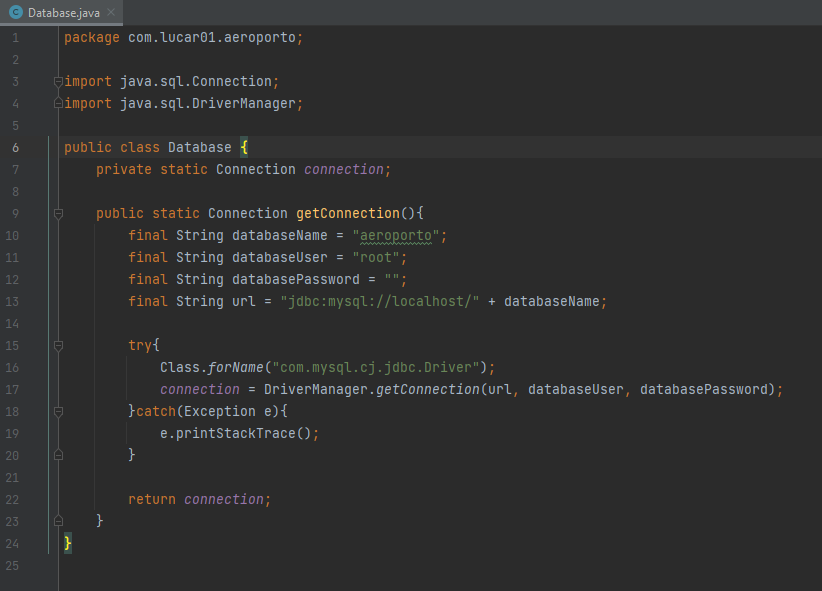
\includegraphics[width=1\textwidth, height=1\textheight, keepaspectratio]{./img/Applicativo/database_class.png}
	\caption{Classe Database}
	\label{fig:database}
\end{figure}

	
	% =========================== CONCLUSIONE =============================================

\newpage

\section{Conclusione}

\textsf{\small Questo conclude questo progetto sulla progettazione di una base di dati riguardante un'infrastruttura aeroportuale.}\\

\textsf{\small Nonostante, immagino che un database di un vero Aeroporto sia molto più grande e complesso di quello che ho fatto io, spero possa esser stato d'aiuto.}\\

\textsf{\small Questo progetto mi ha sicuramente aiutato molto e ha migliorato la mia comprensione dell'architettura, della creazione di un database e della sua interfaccia in un software.}\\

\textsf{\small Grazie per la lettura.}\\

\flushright
%\date{16 Dicembre 2021}\\ %TODO: da modificare la data per quando avrò finito veramente.
\flushleft
\author{Luca Rengo}
	
\end{document}